\chapter{Datenangrundlage und Trainingsvorbereitung} 
\label{chap:datenangrundlage_und_trainingsvorbereitung} 

\section{Datenbasis} 

\subsection{Artikeldaten}
\label{sec:artikeldaten} 

Die Artikeldaten liegen in XML-Dateien vor. 
XML (\textit{Extensible Markup Language}) ist ein standardisiertes Format zur hierarchischen Speicherung und Beschreibung von Informationen, die einem wiederkehrenden Schema folgen \cite{bray2008xml}.
Durch die hierarchische Organisation von XML-Dokumenten können sowohl einfache Stammdaten wie Herstellerinformationen als auch komplexe technische Informationen wie Spannungen, 
Ströme oder Leistungen strukturiert abgebildet werden \cite{bray2008xml}.
Die in den Artikeldaten enthaltenen Informationen, werden im folgenden als \textit{technische Artikeleigenschaften} bezeichnet. 
Zu diesen gehören unter anderen:

\begin{itemize} 
    \item Herstellerinformationen, 
    \item Typnummern, 
    \item Spannungen, 
    \item Ströme, 
    \item Leistungen,  
    \item technische Hinweise, 
    \item Referenzen auf zugehörige Makros. 
\end{itemize} 

Um diese \textit{technische Artikeleigenschaften} anhand des Motorbeispiels aus Kapitel \ref{sec:herleitung} zu veranschaulichen, soll hierfür ein Motor von SEW betrachtet werden.
Abbildung \ref{fig:xml_artikel_motor} zeigt die beispielhafte Struktur eines XML-Artikels für diesen Motor.

\begin{figure}[H] 
    \centering 
    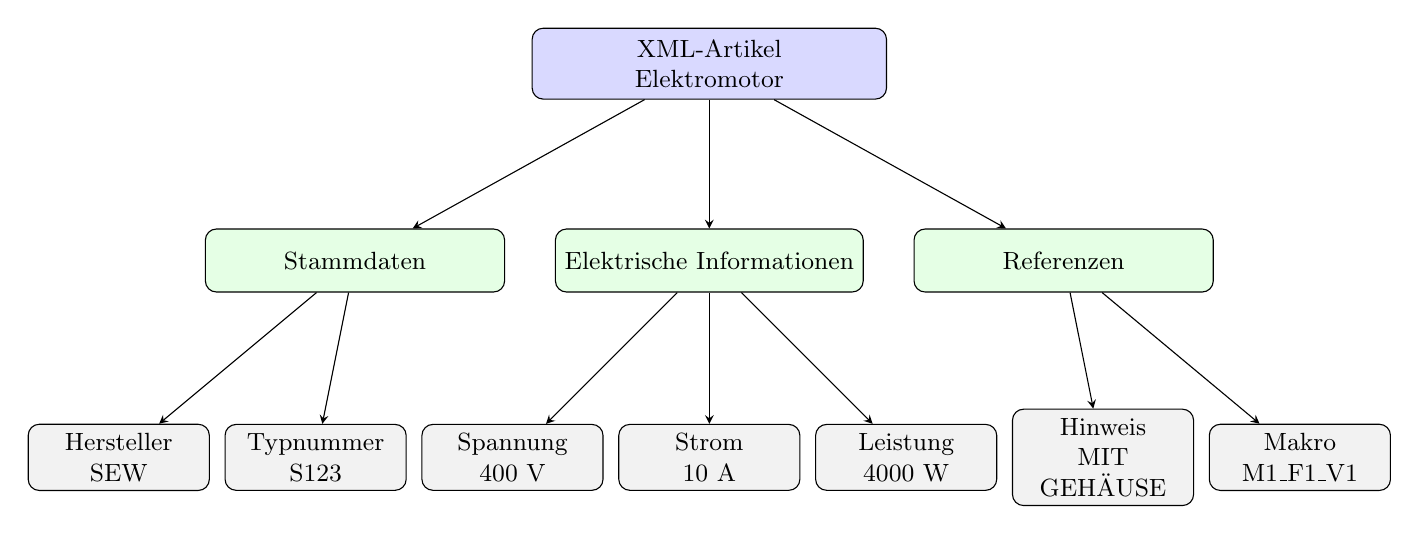
\begin{tikzpicture}[>=stealth, font=\small, 
        every node/.style={align=center}, 
        root/.style={ draw, rounded corners, 
        fill=blue!15, minimum width=4.5cm, minimum height=0.9cm }, 
        category/.style={ draw, rounded corners, fill=green!10, minimum width=3.8cm, minimum height=0.8cm }, 
        feature/.style={ draw, rounded corners, fill=gray!10, minimum width=2.3cm, minimum height=0.8cm, align=center } ] 
        % Wurzel 
        \node[root] (article) at (0,5) {XML-Artikel\\Elektromotor}; 
        % Kategorien 
        \node[category] (master) at (-4.5,2.5) {Stammdaten}; 
        \node[category] (electrical) at (0,2.5) {Elektrische Informationen}; 
        \node[category] (technical) at (4.5,2.5) {Referenzen};
        % Verbindungen 
        \draw[->] (article) -- (master); 
        \draw[->] (article) -- (electrical); 
        \draw[->] (article) -- (technical); 
        % Stammdaten 
        \node[feature] (manu) at (-7.5,0) {Hersteller\\SEW}; 
        \node[feature] (type) at (-5.0,0) {Typnummer\\S123}; 
        \draw[->] (master) -- (manu); 
        \draw[->] (master) -- (type);
        % Elektrische Informationen 
        \node[feature] (voltage) at (-2.5,0) {Spannung\\400 V}; 
        \node[feature] (current) at (0,0) {Strom\\10 A}; 
        \node[feature] (power) at (2.5,0) {Leistung\\4000 W};
        \draw[->] (electrical) -- (voltage); 
        \draw[->] (electrical) -- (current); 
        \draw[->] (electrical) -- (power); 
        % Technische Informationen 
        \node[feature] (ip) at (5.0,0) {Hinweis\\MIT\\GEHÄUSE}; 
        \node[feature] (com) at (7.5,0) {Makro\\M1\_F1\_V1};
        \draw[->] (technical) -- (com); 
        \draw[->] (technical) -- (ip); 
        % Makro
        %\draw[ decorate, decoration={brace,mirror,amplitude=10pt}, thick ] (-8.25,-0.8) -- (8.25,-0.8) node[midway,yshift=-1cm] { \fbox{\strut Zugeordnetes Motor-Makro} };
    \end{tikzpicture} 
    \caption{Beispielhafte Struktur eines XML-Artikels für einen Elektromotor. Die hierarchische Organisation ermöglicht die strukturierte Speicherung von \textit{technischen Artikeleigenschaften} eines Motors nach einem vorgegebenen Schema.} 
    \label{fig:xml_artikel_motor}
\end{figure}

\subsection{Makrodaten} 

Neben den Artikeln werden die zugehörigen Makros analysiert. Die Makros sind im .ema-Format gespeichert. 
Dieses Format entspricht ebenfalls einem XML-Schema, das Informationen über die Makros in einem einheitlichen Schema strukturiert abbildet.

Diese Informationen werden im folgenden als \textit{technische Makroeigenschaften} bezeichnet. 

Hierzu zählen: 

\begin{itemize} 
    \item Anschlussstrukturen,  
    \item Makrovarianten,   
    \item Bezeichnungen. 
\end{itemize} 


Die Bezeichnung eines Makros wird dabei nach folgendem Muster aufgebaut: Klasse-Familie-Variante (z.\,B. M1\_F1\_V1)
Die Klasse gibt die Art des Makros selbst an, die Familie beschreibt eine Unterkategorie des Makros und die Variante kennzeichnet unterschiedliche Ausführungen innerhalb dieser Familie.
Im Fall des Motorbeispiels aus Kapitel \ref{sec:herleitung} lässt sich die Bezeichnung M1\_F1\_V1 wie folgt interpretieren:

\begin{itemize}
    \item  M1: Motor
    \item  F1: Gleichstrommotor
    \item  V1: Mit Kühlung
\end{itemize}

Die Abbildung \ref{fig:ema_motor_macro} gibt die Struktur eines Motor-Makros im .ema-Format wieder.

\begin{figure}[H] 
    \centering 
    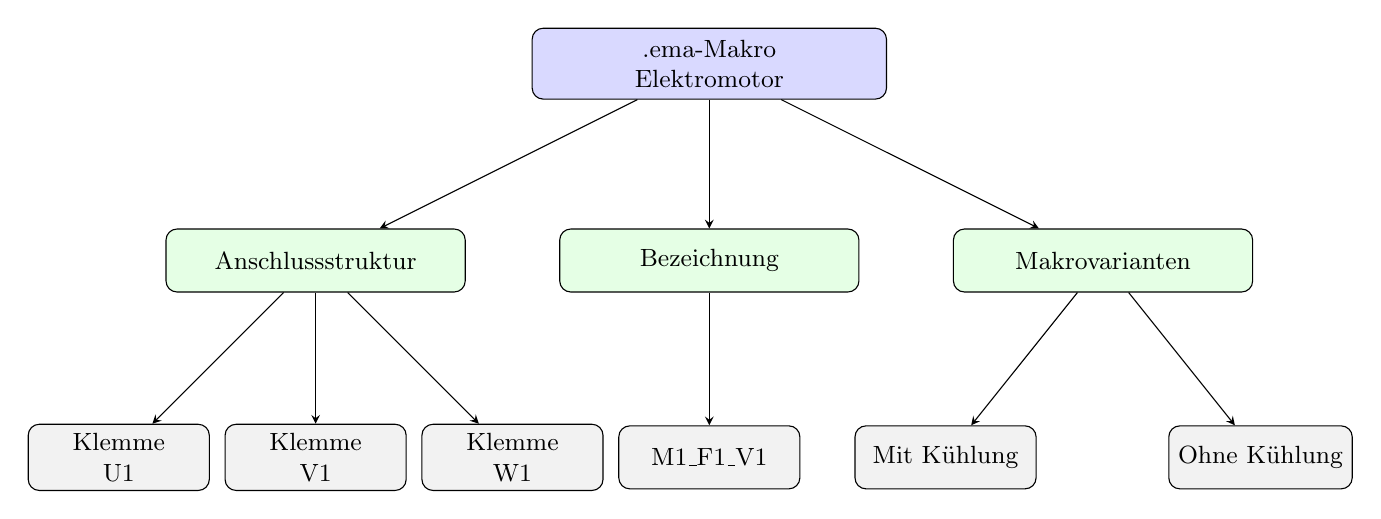
\begin{tikzpicture}[>=stealth, font=\small, 
        every node/.style={align=center}, 
        root/.style={ draw, rounded corners, 
        fill=blue!15, minimum width=4.5cm, minimum height=0.9cm }, 
        category/.style={ draw, rounded corners, fill=green!10, minimum width=3.8cm, minimum height=0.8cm }, 
        feature/.style={ draw, rounded corners, fill=gray!10, minimum width=2.3cm, minimum height=0.8cm, align=center } ] 
        % Wurzel 
        \node[root] (macro) at (0,5) {.ema-Makro\\Elektromotor}; 
        % Kategorien 
        \node[category] (terminal) at (-5.0,2.5) {Anschlussstruktur}; 
        \node[category] (function) at (0,2.5) {Bezeichnung}; 
        \node[category] (variant) at (5.0,2.5) {Makrovarianten}; 
        % Verbindungen 
        \draw[->] (macro) -- (terminal); 
        \draw[->] (macro) -- (function); 
        \draw[->] (macro) -- (variant); 
        % Anschlussstruktur 
        \node[feature] (u1) at (-7.5,0) {Klemme\\U1}; 
        \node[feature] (v1) at (-5.0,0) {Klemme\\V1}; 
        \node[feature] (w1) at (-2.5,0) {Klemme\\W1}; 
        \draw[->] (terminal) -- (u1); 
        \draw[->] (terminal) -- (v1); 
        \draw[->] (terminal) -- (w1); 
        % Bezeichnung 
        \node[feature] (motor) at (0,0) {M1\_F1\_V1}; 
        \draw[->] (function) -- (motor); 
        % Varianten 
        \node[feature] (left) at (3.0,0) {Mit Kühlung}; 
        \node[feature] (right) at (7.0,0) {Ohne Kühlung}; 
        \draw[->] (variant) -- (left); 
        \draw[->] (variant) -- (right); 
    \end{tikzpicture} 
    \caption{Beispielhafte Struktur eines Motor-Makros im .ema-Format. Das Makro beschreibt die technische Umsetzung eines Elektromotors im Schaltplan und enthält Informationen zu Anschlussstrukturen, Bezeichnungen und Makrovarianten.} 
    \label{fig:ema_motor_macro} 
\end{figure}

\subsection{Artikel-Makro-Zuordnungen}
\label{sec:artikel_macro_zuordnungen}

Die Zuordnung von Artikel zu Makro erfolgt durch die Referenzierung des Makros über die \textit{technische Artikeleigenschaft} \texttt{P\_ARTICLE\_MACRO}.
Diese Zuordnung kann als n zu 1 Beziehung betrachtet werden, da mehrere Artikel auf dasselbe Makro verweisen können. Mehrer Artikel welche im Schaltplan dasselbe Makro repräsentieren, werden im folgenden als \textit{Artikelgruppe} bezeichnet.
Beispielsweise können einem Makro eines Motors mehrere Artikel unterschiedlicher Hersteller zugeordnet werden.

Bildlich kann dies durch folgende Abbildung \ref{fig:artikel_macro_n_zu_1} dargestellt werden: 

\begin{figure}[H] 
    \centering 
    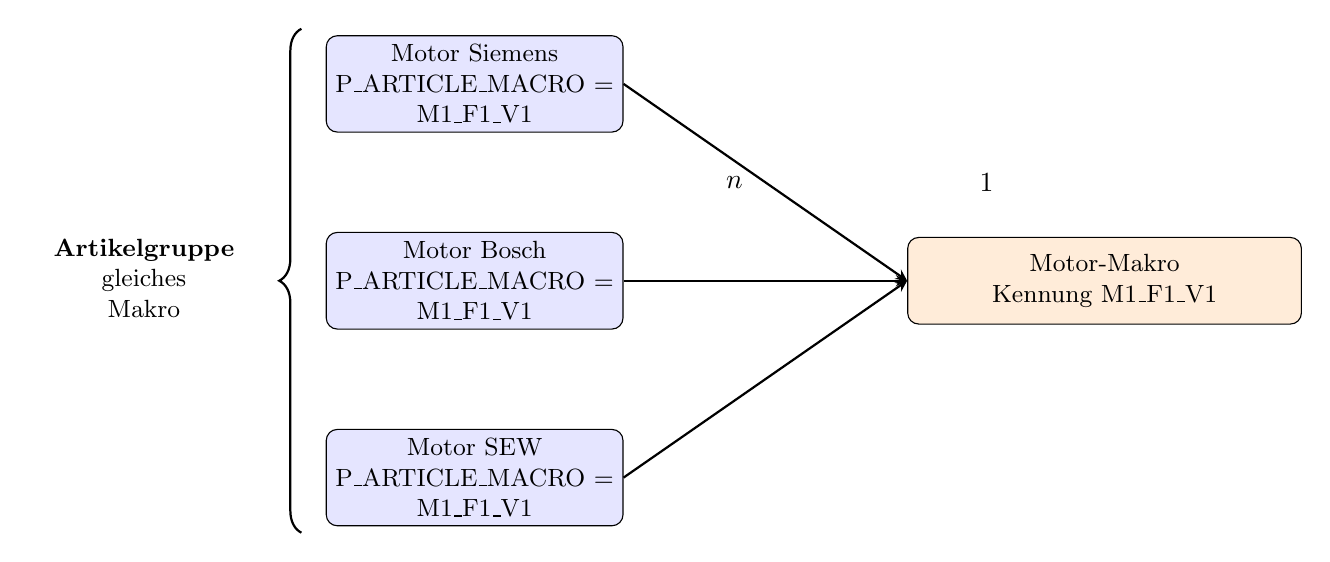
\begin{tikzpicture}[ >=stealth, font=\small, 
        article/.style={ draw, rounded corners, fill=blue!10, minimum width=3.2cm, minimum height=1.2cm, align=center },
        macro/.style={ draw, rounded corners, fill=orange!15, minimum width=5cm, minimum height=1.1cm, align=center } ] 
        % Artikel 
        \node[article] (a1) at (0, 2.5) { Motor Siemens\\ P\_ARTICLE\_MACRO =\\ M1\_F1\_V1 }; 
        \node[article] (a2) at (0, 0) { Motor Bosch\\ P\_ARTICLE\_MACRO =\\ M1\_F1\_V1 }; 
        \node[article] (a3) at (0,-2.5) { Motor SEW\\ P\_ARTICLE\_MACRO =\\ M1\_F1\_V1 }; 
        % Makro 
        \node[macro] (m1) at (8,0) {Motor-Makro\\Kennung M1\_F1\_V1}; 
        % Verbindungen 
        \draw[->,thick] (a1.east) -- (m1.west); 
        \draw[->,thick] (a2.east) -- (m1.west); 
        \draw[->,thick] (a3.east) -- (m1.west); 
        % Kardinalitäten 
        \node[font=\bfseries] at (3.3,1.25) {$n$}; 
        \node[font=\bfseries] at (6.5,1.25) {$1$}; 
        % Artikelgruppe 
        \draw[ decorate, decoration={brace,mirror,amplitude=8pt}, thick ] (-2.2,3.2) -- (-2.2,-3.2) node[midway,xshift=-2.0cm] { \begin{tabular}{c} \textbf{Artikelgruppe}\\ gleiches\\ Makro \end{tabular} };
    \end{tikzpicture} 
    \caption{Beispiel einer n:1-Beziehung zwischen Artikeln und Makros. Mehrere Artikel verweisen über die Eigenschaft \texttt{P\_ARTICLE\_MACRO} auf dasselbe Makro.} 
    \label{fig:artikel_macro_n_zu_1} 
\end{figure}


\section{Datenaufbereitung} 
\label{sec:datenaufbereitung}

Die vorliegende Struktur der Daten im XML-Format hat den Vorteil, dass Informationen nicht manuell ausgelesen und weiterverarbeitet werden müssen.
Die Vorbereitung der Daten kann somit automatisiert erfolgen, sodass eine nachvollziehbare und reproduzierbare Vorbereitung der Daten gewährleistet werden kann.
Diese Vorbereitung der Daten wird im weiteren Verlauf als \textit{Datenaufbereitung} bezeichnet. 

Die in Kapitel \ref{sec:modellansätze} beschriebenen Modellansätze lernen statistische Zusammenhänge zwischen den Eingabedaten (Artikel) und den Ausgabedaten (Makros).
Enthalten diese Daten fehlerhafte, unvollständige oder widersprüchliche Informationen, 
werden diese vom Modell während des Lernprozesses übernommen und können die Qualität des Modells negativ beeinflussen \cite{emmanuel2021missing,hastie2009elements}. 
Das Ziel der \textit{Datenaufbereitung} besteht daher darin, die Qualität der Datenbasis zu erhöhen und gleichzeitig Störeinflüsse zu reduzieren, um eine zuverlässige Grundlage für den Lernprozess eines Modells zu schaffen.

\subsection{Entfernung unvollständiger Artikel- und Makrodaten}
\label{sec:entfernen_unvollständiger_artikel_und_makrodaten}

In diesem Schritt werden alle Artikel entfernt, die unvollständige Informationen enthalten. 
Fehlende \textit{technischen Artikeleigenschaften} sind Informationslücken, welche die Vollständigkeit der Daten beeinträchtigen. Dies kann zu einer Verschlechterung der Modellleistung führen und muss daher bereits während der \textit{Datenaufbereitung} behandelt werden \cite{emmanuel2021missing}.
Angenommen, ein unvollständiger Motor-Artikel enthält keine Angaben zur Spannung, dann wird bei einem späteren Lernprozess diese Informationslücke vom Modell übernommen. Wenn dann eine Anfrage an das Modell gestellt wird, welche diesem "spannungslosen" Motor-Artikel entspricht, kann das Modell diesen Artikel nicht korrekt zuordnen, 
da die notwendigen Informationen "Spannung" zum Erkennen dieses Artikels fehlt.

Abbildung \ref{fig:unvollstaendige_daten} verdeutlicht die Unterscheidung zwischen vollständigen und unvollständigen Artikeldaten:

\begin{figure}[H] 
    \centering 
    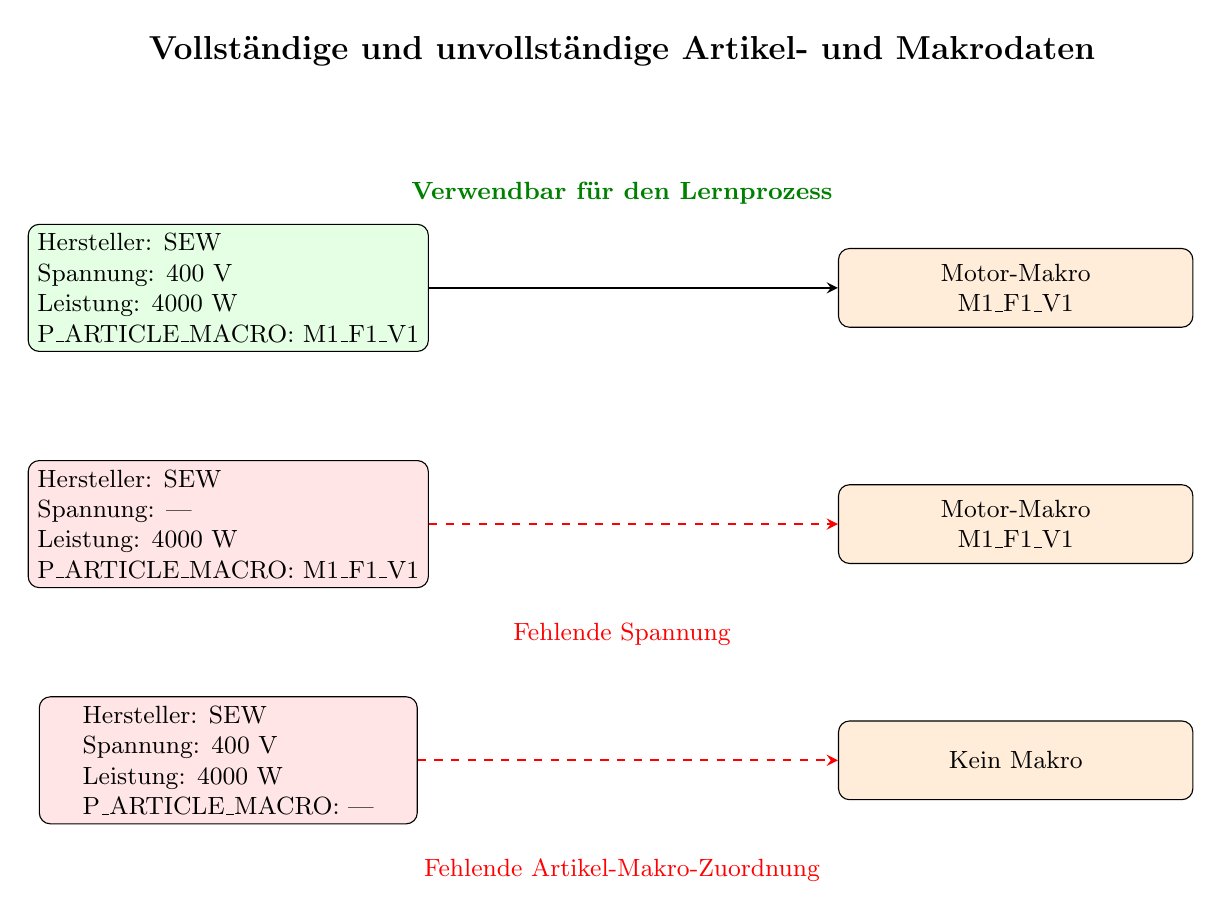
\begin{tikzpicture}[ >=stealth, font=\small, 
        valid/.style={ draw, rounded corners, fill=green!10, minimum width=4.8cm, minimum height=1.2cm, align=left }, 
        invalid/.style={ draw, rounded corners, fill=red!10, minimum width=4.8cm, minimum height=1.2cm, align=left }, 
        macro/.style={ draw, rounded corners, fill=orange!15, minimum width=4.5cm, minimum height=1.0cm, align=center } ] 
        
        %%%%%%%%%%%%%%%%%%%%%%%%%%%%%%%%%%%%%%%%%%%%%%%%% % Überschrift %%%%%%%%%%%%%%%%%%%%%%%%%%%%%%%%%%%%%%%%%%%%%%%%% 
        
        \node[font=\bfseries\large] at (0,5) {Vollständige und unvollständige Artikel- und Makrodaten}; 
        
        %%%%%%%%%%%%%%%%%%%%%%%%%%%%%%%%%%%%%%%%%%%%%%%%% % Gültiger Artikel %%%%%%%%%%%%%%%%%%%%%%%%%%%%%%%%%%%%%%%%%%%%%%%%% 
        
        \node[valid] (a1) at (-5,2) { Hersteller: SEW\\ Spannung: 400 V\\ Leistung: 4000 W\\ P\_ARTICLE\_MACRO: M1\_F1\_V1 }; 
        \node[macro] (m1) at (5,2) {Motor-Makro\\M1\_F1\_V1}; \draw[->,thick] (a1.east) -- (m1.west); \node[text=green!50!black] at (0,3.2) {\textbf{Verwendbar für den Lernprozess}}; 
        
        %%%%%%%%%%%%%%%%%%%%%%%%%%%%%%%%%%%%%%%%%%%%%%%%% % Ungültiger Artikel 1 %%%%%%%%%%%%%%%%%%%%%%%%%%%%%%%%%%%%%%%%%%%%%%%%% 
        
        \node[invalid] (a2) at (-5,-1) { Hersteller: SEW\\ Spannung: ---\\ Leistung: 4000 W\\ P\_ARTICLE\_MACRO: M1\_F1\_V1 }; 
        \node[macro] (m2) at (5,-1) {Motor-Makro\\M1\_F1\_V1}; 
        \draw[dashed,red,thick,->] (a2.east) -- (m2.west); 
        \node[text=red] at (0,-2.4) {Fehlende Spannung}; 

        %%%%%%%%%%%%%%%%%%%%%%%%%%%%%%%%%%%%%%%%%%%%%%%%% % Ungültiger Artikel 2 %%%%%%%%%%%%%%%%%%%%%%%%%%%%%%%%%%%%%%%%%%%%%%%%% 
        \node[invalid] (a3) at (-5,-4) { Hersteller: SEW\\ Spannung: 400 V\\ Leistung: 4000 W\\ P\_ARTICLE\_MACRO: --- }; 
        \node[macro] (m3) at (5,-4) {Kein Makro}; 
        \draw[dashed,red,thick,->] (a3.east) -- (m3.west); 
        \node[text=red] at (0,-5.4) {Fehlende Artikel-Makro-Zuordnung}; 
    \end{tikzpicture} 
    \caption{Beispiel für vollständige und unvollständige Artikel- und Makrodaten. Fehlende \textit{technischen Artikeleigenschaften} sorgen für Informationslücken im späteren Lernprozess und werden daher aus den Artikel- und Makrodaten entfernt.} 
    \label{fig:unvollstaendige_daten} 
\end{figure}

\subsection{Entfernung redundanter Artikel}
\label{sec:entfernung_redundanter_artikel}

Hierbei werden identische Artikel identifiziert, welche dieselben \textit{technischen Artikeleigenschaften} aufweisen. 
Identische Artikel, welche in mehrfacher Ausführung auftreten, führen dazu, dass diese gegenüber anderen Artikeln, welche in einzelner Ausführung auftreten, 
übergewichtet werden. In einem späteren Lernprozess wird hierdurch das Wissen eines Modells verzerrt, indem 
das Modell ein Vorurteil auf übergewichtete Artikel erlernt, welche bei neuen Anfragen bevorzugt für die Vorhersage verwendet werden \cite{hastie2009elements,sabzekar2021noiseaware}.

Abbildung \ref{fig:redundante_daten} veranschaulicht die Übergewichtung redundanter Motor-Artikel. Nach der Bereinigung werden identische Artikel entfernt, sodass jedes Exemplar nur einmal vorkommt.

\begin{figure}[H] 
    \centering 
    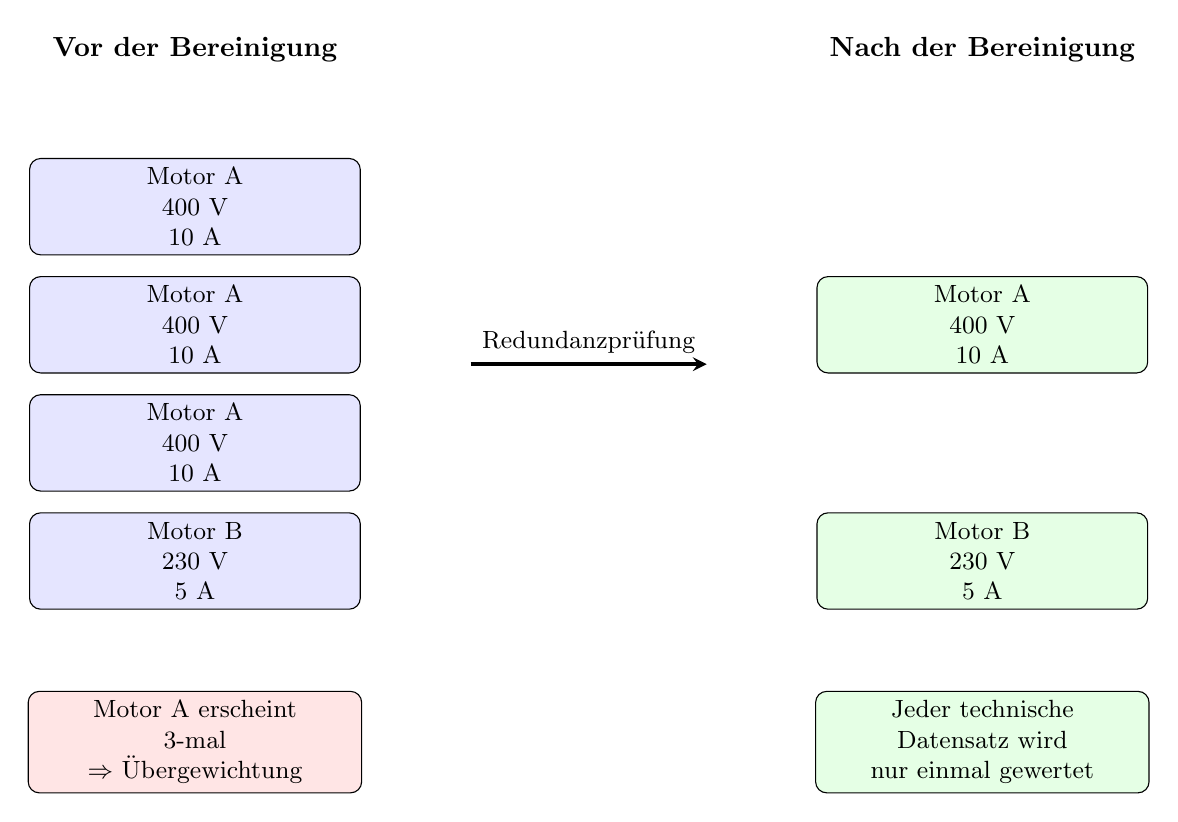
\begin{tikzpicture}[ >=stealth, font=\small, 
        article/.style={ draw, rounded corners, fill=blue!10, minimum width=4.2cm, minimum height=0.9cm, align=center }, 
        clean/.style={ draw, rounded corners, fill=green!10, minimum width=4.2cm, minimum height=0.9cm, align=center } ] 
        
        %%%%%%%%%%%%%%%%%%%%%%%%%%%%%%%%%%%%%%%%%%%%%%%%% % Vor Bereinigung %%%%%%%%%%%%%%%%%%%%%%%%%%%%%%%%%%%%%%%%%%%%%%%%% 
        
        \node[font=\bfseries] at (-5,4.5) {Vor der Bereinigung}; 
        \node[article] (a1) at (-5,2.5) {Motor A\\400 V\\10 A}; 
        \node[article] (a2) at (-5,1.0) {Motor A\\400 V\\10 A}; 
        \node[article] (a3) at (-5,-0.5) {Motor A\\400 V\\10 A}; 
        \node[article] (a4) at (-5,-2.0) {Motor B\\230 V\\5 A}; 
        
        % Gewichtung 
        
        \node[ draw, fill=red!10, rounded corners, text width=4cm, align=center ] at (-5,-4.3) { Motor A erscheint\\ 3-mal\\ $\Rightarrow$ Übergewichtung }; 
        
        %%%%%%%%%%%%%%%%%%%%%%%%%%%%%%%%%%%%%%%%%%%%%%%%% % Pfeil %%%%%%%%%%%%%%%%%%%%%%%%%%%%%%%%%%%%%%%%%%%%%%%%% 
        
        \draw[->,very thick] (-1.5,0.5) -- (1.5,0.5) node[midway,above] {Redundanzprüfung}; 
        
        %%%%%%%%%%%%%%%%%%%%%%%%%%%%%%%%%%%%%%%%%%%%%%%%% % Nach Bereinigung %%%%%%%%%%%%%%%%%%%%%%%%%%%%%%%%%%%%%%%%%%%%%%%%% 
        
        \node[font=\bfseries] at (5,4.5) {Nach der Bereinigung}; 
        \node[clean] (c1) at (5,1.0) {Motor A\\400 V\\10 A}; 
        \node[clean] (c2) at (5,-2.0) {Motor B\\230 V\\5 A}; 
        \node[ draw, fill=green!10, rounded corners, text width=4cm, align=center ] at (5,-4.3) { Jeder technische\\ Datensatz wird\\ nur einmal gewertet }; 
        
    \end{tikzpicture} 
    \caption{Auswirkung redundanter Artikel. Mehrfach vorhandene Daten erhöhen künstlich deren Gewichtung. Durch die Entfernung redundanter Daten wird diese Übergewichtung verhindert.} 
    \label{fig:redundante_daten} 
\end{figure}


\subsection{Entfernen nicht nutzbarer Metadaten}
\label{sec:entfernen_nicht_nutzbarer_metadaten}

Metadaten sind Informationen über Daten, die nicht direkt mit dem Inhalt dieser Daten zusammenhängen. Beispiele hierfür sind Erstellungsdatum, Änderungsdatum oder Autor. 
Diese Metadaten sind für die Erkennung von Unterschieden zwischen \textit{technischen Artikeleigenschaften} nicht relevant und werden als Rauschen bezeichnet.
Dieses Rauschen kann als Informationsüberflutung betrachtet werden, was dazu führt, dass ein Modell später Wissen über irrelevante Informationen erlernt und dadurch die Erkennung relevanter \textit{technischen Artikeleigenschaften} erschwert wird \cite{sabzekar2021noiseaware}.

Anhand der Abbildung \ref{fig:metadaten_filter} soll verdeutlicht werden, wie sich Metadaten von relevanten \textit{technischen Eigenschaften} unterscheiden:

\begin{figure}[H] 
    \centering 
    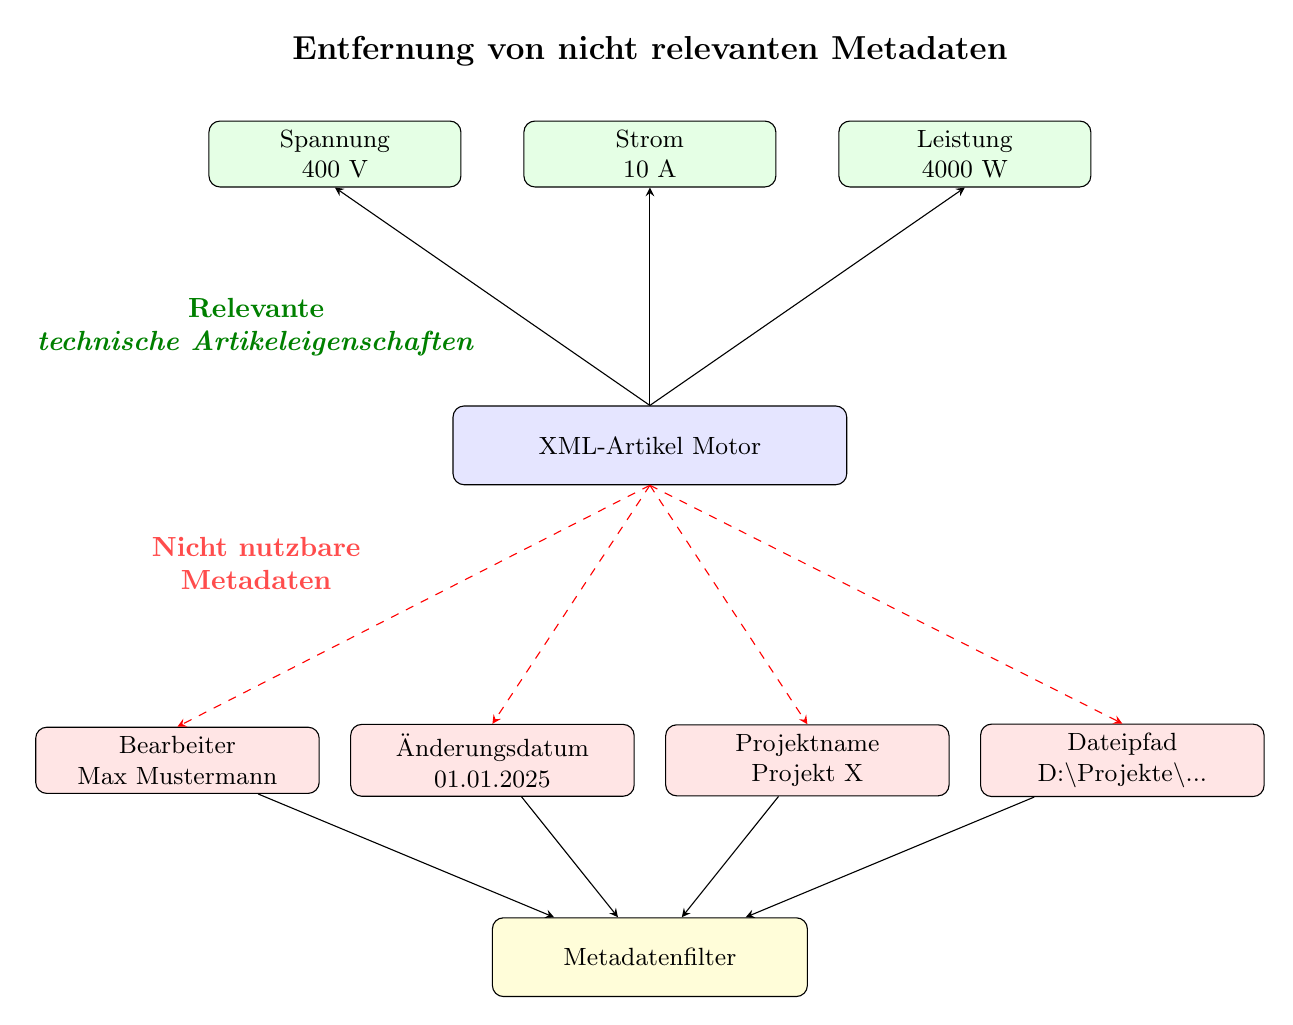
\begin{tikzpicture}[ >=stealth, font=\small, 
        relevant/.style={ draw, rounded corners, fill=green!10, minimum width=3.2cm, minimum height=0.8cm, align=center }, 
        metadata/.style={ draw, rounded corners, fill=red!10, minimum width=3.6cm, minimum height=0.8cm, align=center }, 
        result/.style={ draw, rounded corners, fill=blue!10, minimum width=5cm, minimum height=1cm, align=center } ] 
        
        %%%%%%%%%%%%%%%%%%%%%%%%%%%%%%%%%%%%%%%%%%%%%%%%% % Titel %%%%%%%%%%%%%%%%%%%%%%%%%%%%%%%%%%%%%%%%%%%%%%%%% 
        
        \node[font=\bfseries\large] at (0,6.5) {Entfernung von nicht relevanten Metadaten}; 
        
        %%%%%%%%%%%%%%%%%%%%%%%%%%%%%%%%%%%%%%%%%%%%%%%%% % XML-Artikel %%%%%%%%%%%%%%%%%%%%%%%%%%%%%%%%%%%%%%%%%%%%%%%%% 
        \node[result] (article) at (0,1.5) {XML-Artikel Motor}; 
        %%%%%%%%%%%%%%%%%%%%%%%%%%%%%%%%%%%%%%%%%%%%%%%%% % Relevante Informationen %%%%%%%%%%%%%%%%%%%%%%%%%%%%%%%%%%%%%%%%%%%%%%%%% 
        \node[ font=\bfseries, text=green!50!black, align=center ] at (-5,3.0) {Relevante\\\textit{technische Artikeleigenschaften}}; 
        \node[relevant] (v) at (-4,5.2) {Spannung\\400 V}; 
        \node[relevant] (i) at (0,5.2) {Strom\\10 A}; 
        \node[relevant] (p) at (4,5.2) {Leistung\\4000 W}; 
        \draw[->] (article.north) -- (v.south); 
        \draw[->] (article.north) -- (i.south); 
        \draw[->] (article.north) -- (p.south); 
        %%%%%%%%%%%%%%%%%%%%%%%%%%%%%%%%%%%%%%%%%%%%%%%%% % Metadaten %%%%%%%%%%%%%%%%%%%%%%%%%%%%%%%%%%%%%%%%%%%%%%%%% 
        \node[ font=\bfseries, text=red!70, align=center ] at (-5,0.0) {Nicht nutzbare\\Metadaten}; 
        \node[metadata] (author) at (-6,-2.5) {Bearbeiter\\Max Mustermann}; 
        \node[metadata] (date) at (-2,-2.5) {Änderungsdatum\\01.01.2025}; 
        \node[metadata] (project) at (2,-2.5) {Projektname\\Projekt X}; 
        \node[metadata] (path) at (6,-2.5) {Dateipfad\\D:\textbackslash Projekte\textbackslash ...}; 
        \draw[->,red,dashed] (article.south) -- (author.north); 
        \draw[->,red,dashed] (article.south) -- (date.north); 
        \draw[->,red,dashed] (article.south) -- (project.north); 
        \draw[->,red,dashed] (article.south) -- (path.north); 
        %%%%%%%%%%%%%%%%%%%%%%%%%%%%%%%%%%%%%%%%%%%%%%%%% % Filter %%%%%%%%%%%%%%%%%%%%%%%%%%%%%%%%%%%%%%%%%%%%%%%%% 
        \node[ draw, rounded corners, fill=yellow!15, minimum width=4cm, minimum height=1cm ] (filter) at (0,-5) {Metadatenfilter}; 
        \draw[->] (author) -- (filter); 
        \draw[->] (date) -- (filter); 
        \draw[->] (project) -- (filter); 
        \draw[->] (path) -- (filter);

        \end{tikzpicture} 
        \caption{Nicht relevanten Metadaten. \textit{Technische Artikeleigenschaften} bleiben erhalten, während Metadaten ohne relevanten Informationsgehalt entfernt werden.} 
        \label{fig:metadaten_filter} 
        \end{figure}


\subsection{Normaliserung von Einheiten} 
\label{sec:normaliserung_von_einheiten}

Die \textit{technischen Artikeleigenschaften} liegen in unterschiedlichen Einheiten oder Schreibweisen vor.
Ohne zusätzliches Wissen über die einzelnen Schreibweisen der \textit{technischen Artikeleigenschaften} sind diese nicht direkt vergleichbar. 
Die Vereinheitlichung der \textit{technischen Artikeleigenschaften} reduziert Variationen in den Artikeldaten und bildet die Basis für eine belastbare Bewertung des Modells \cite{hastie2009elements}. 
Angenommen in mehreren Artikeln steht die Spannung einmal als 24 V, einmal als 24VDC und einmal als 0,024 kV, so handelt es sich um denselben Wert, der jedoch unterschiedlich dargestellt wird.
Wird ein Modell das eine Spannung von 24 V ausgibt, mit einer Spannung von 24VDC oder 0,024 kV bewertet, wird fälschlicherweise ein Unterschied angenommen, obwohl es sich um dieselbe Spannung handelt.
Deswegen werden die \textit{technischen Artikeleigenschaften} aus den Artikeln auf gemeinsame Basiseinheiten normiert.

Folgende Abbildung \ref{fig:einheitennormalisierung} soll dazu diesen Sachverhalt zu veranschaulichen:

\begin{figure}[H] 
    \centering 
    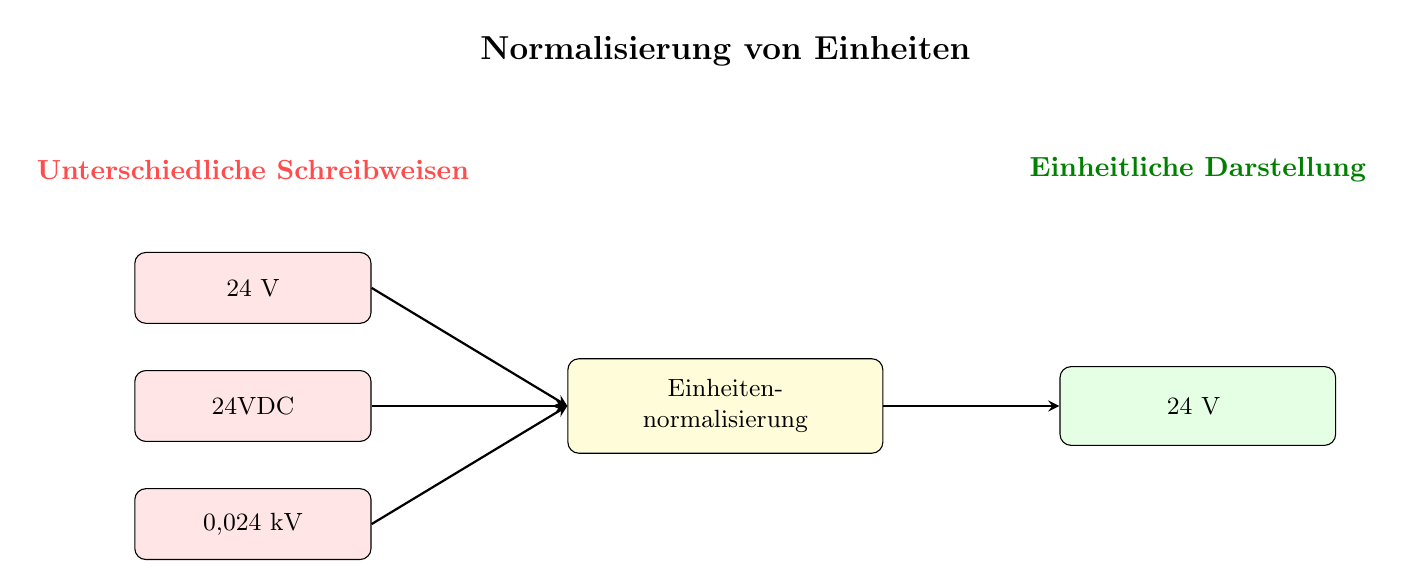
\begin{tikzpicture}[ >=stealth, font=\small, 
        raw/.style={ draw, rounded corners, fill=red!10, minimum width=3.0cm, minimum height=0.9cm, align=center }, 
        process/.style={ draw, rounded corners, fill=yellow!15, minimum width=4.0cm, minimum height=1.2cm, align=center }, 
        norm/.style={ draw, rounded corners, fill=green!10, minimum width=3.5cm, minimum height=1.0cm, align=center } ] 
        
        %%%%%%%%%%%%%%%%%%%%%%%%%%%%%%%%%%%%%%%%%%%%%%%%% % Titel %%%%%%%%%%%%%%%%%%%%%%%%%%%%%%%%%%%%%%%%%%%%%%%%% 
        
        \node[font=\bfseries\large] at (0,5) {Normalisierung von Einheiten}; 
        
        %%%%%%%%%%%%%%%%%%%%%%%%%%%%%%%%%%%%%%%%%%%%%%%%% % Ausgangswerte %%%%%%%%%%%%%%%%%%%%%%%%%%%%%%%%%%%%%%%%%%%%%%%%% 
        
        \node[font=\bfseries,text=red!70] at (-6,3.5) {Unterschiedliche Schreibweisen}; 
        \node[raw] (v1) at (-6,2) {24 V}; 
        \node[raw] (v2) at (-6,0.5) {24VDC}; 
        \node[raw] (v3) at (-6,-1) {0,024 kV}; 
        
        %%%%%%%%%%%%%%%%%%%%%%%%%%%%%%%%%%%%%%%%%%%%%%%%% % Prozess %%%%%%%%%%%%%%%%%%%%%%%%%%%%%%%%%%%%%%%%%%%%%%%%% 
        
        \node[process] (normprocess) at (0,0.5) { Einheiten-\\ normalisierung }; 
        \draw[->,thick] (v1.east) -- (normprocess.west); 
        \draw[->,thick] (v2.east) -- (normprocess.west); 
        \draw[->,thick] (v3.east) -- (normprocess.west); 
        %%%%%%%%%%%%%%%%%%%%%%%%%%%%%%%%%%%%%%%%%%%%%%%%% % Ergebnis %%%%%%%%%%%%%%%%%%%%%%%%%%%%%%%%%%%%%%%%%%%%%%%%% 
        \node[font=\bfseries,text=green!50!black] at (6,3.5) {Einheitliche Darstellung}; 
        \node[norm] (result) at (6,0.5) { 24 V }; 
        \draw[->,thick] (normprocess.east) -- (result.west); 
    \end{tikzpicture} 
    \caption{Beispiel für die Normalisierung technischer Einheiten. Unterschiedliche Schreibweisen derselben Spannung werden in eine einheitliche Darstellung überführt, wodurch die Vergleichbarkeit dieser Einheiten verbessert wird.} 
    \label{fig:einheitennormalisierung} 
\end{figure}

\subsection{Erstellung von Klassifikationen}
\label{sec:erstellung_von_klassifikationen}

Die Vorhandenen \textit{technischen Artikeleigenschaften} liegen in unterschiedlichen Wertebereichen vor. 
Dieses Wissen über die Wertebereiche ermöglicht es, die \textit{technischen Artikeleigenschaften} zu Klassifikationen zusammenzufassen.
Eine Klassifikation fasst kontinuierliche Wertebereiche wie 22 Volt - 26 Volt zu einzelnen Kategorien zusammen \cite{fayyad1993discretization}.
Diese Klassifikationen stellen ein zusätzliches Wissen in den \textit{technischen Artikeleigenschaften} dar, welches für die Vergleichbarkeit mehrerer Artikel nützlich ist.
Um dies zu Verdeutlichen folgendes konkretes Beispiel: Die Spannung eines Artikels wird in die Kategorien \textit{niedrige Spannung}, \textit{mittlere Spannung} und \textit{hohe Spannung} eingeteilt werden.
Dabei werden Spannungen bis 100 V der Kategorie \textit{niedrige Spannung}, Spannungen von 101 V bis 1000 V der Kategorie \textit{mittlere Spannung} und Spannungen über 1000 V der Kategorie \textit{hohe Spannung} zugeordnet.
Diese Kategorien erzeugen die zusätzliche Information, dass \textit{technische Artikeleigenschaften} eines Artikels trotz einer Streuung von Werten um einen Mittelwert in eine bestimmte Kategorie fallen.
Ein späteres Modell kann diese Information nutzen, um Makros zu empfehlen, deren Artikel nicht exakt den gleichen Wert haben wie der Artikel aus der Anfrage. 
Somit kann ein Makro empfohlen werden, dass einen Artikel mit 48 V als Grundlage enthält, obwohl der Artikel aus der Anfrage 50 V aufweist. 
Die entstehenden Kategorien werden als neue \textit{technische Artikeleigenschaft} in den Artikeln gespeichert.

Die folgende Abbildung \ref{fig:spannungsklassifikation} zeigt, wie die Klassifikation von Spannungen dargestellt wird: 

\begin{figure}[H] 
    \centering 
    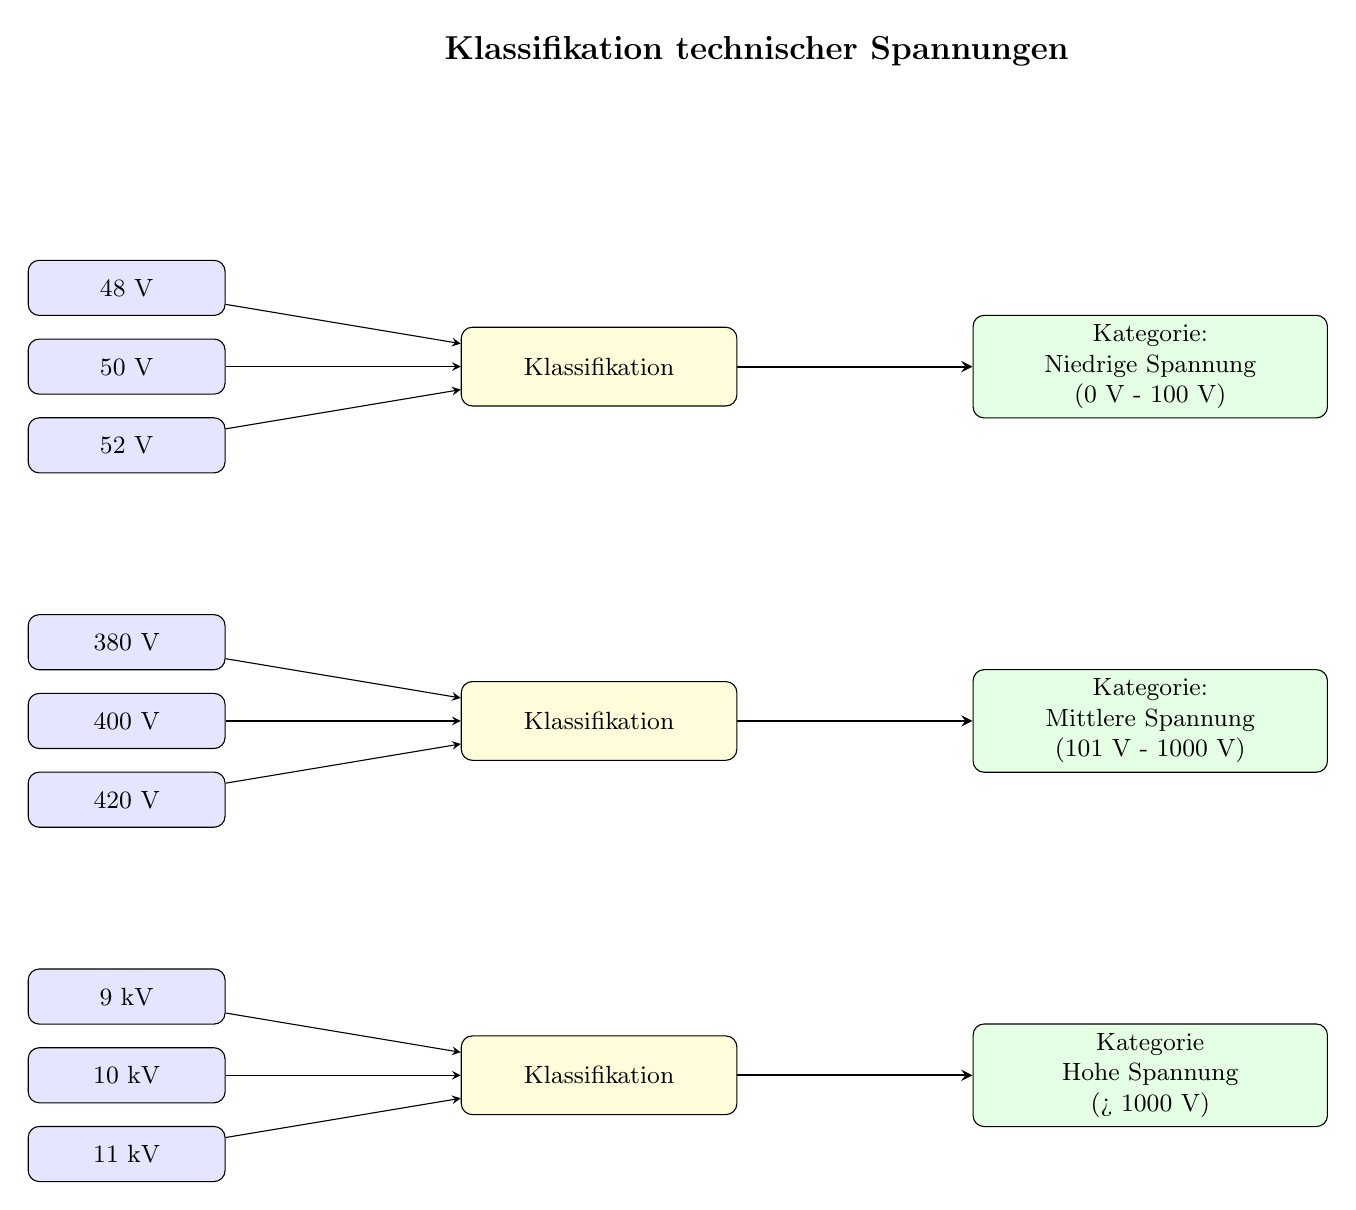
\begin{tikzpicture}[ >=stealth, font=\small, 
        value/.style={ draw, rounded corners, fill=blue!10, minimum width=2.5cm, minimum height=0.7cm, align=center }, 
        class/.style={ draw, rounded corners, fill=green!10, minimum width=4.5cm, minimum height=1.0cm, align=center }, 
        process/.style={ draw, rounded corners, fill=yellow!15, minimum width=3.5cm, minimum height=1cm, align=center },
        macro/.style={ draw, rounded corners, fill=orange!15, minimum width=4.5cm, minimum height=1cm, align=center } ] 
        
        %%%%%%%%%%%%%%%%%%%%%%%%%%%%%%%%%%%%%%%%%%%%%%%%% % Titel %%%%%%%%%%%%%%%%%%%%%%%%%%%%%%%%%%%%%%%%%%%%%%%%% 
        
        \node[font=\bfseries\large] at (0,9) {Klassifikation technischer Spannungen}; 
        
        %%%%%%%%%%%%%%%%%%%%%%%%%%%%%%%%%%%%%%%%%%%%%%%%% % Niedrige Spannung %%%%%%%%%%%%%%%%%%%%%%%%%%%%%%%%%%%%%%%%%%%%%%%%% 
        
        \node[value] (lv1) at (-8,6) {48 V}; 
        \node[value] (lv2) at (-8,5) {50 V}; 
        \node[value] (lv3) at (-8,4) {52 V}; 
        \node[process] (c1) at (-2,5) {Klassifikation}; 
        \node[class] (low) at (5,5) { Kategorie:\\ Niedrige Spannung\\ (0 V - 100 V) }; 
        
        \draw[->] (lv1) -- (c1); 
        \draw[->] (lv2) -- (c1); 
        \draw[->] (lv3) -- (c1); 
        \draw[->,thick] (c1) -- (low); 
        
        %%%%%%%%%%%%%%%%%%%%%%%%%%%%%%%%%%%%%%%%%%%%%%%%% % Mittlere Spannung %%%%%%%%%%%%%%%%%%%%%%%%%%%%%%%%%%%%%%%%%%%%%%%%% 
        
        \node[value] (mv1) at (-8,1.5) {380 V}; 
        \node[value] (mv2) at (-8,0.5) {400 V}; 
        \node[value] (mv3) at (-8,-0.5) {420 V}; 
        \node[process] (c2) at (-2,0.5) {Klassifikation}; 
        \node[class] (medium) at (5,0.5) { Kategorie:\\ Mittlere Spannung\\ (101 V - 1000 V) }; 
        
        \draw[->] (mv1) -- (c2); 
        \draw[->] (mv2) -- (c2); 
        \draw[->] (mv3) -- (c2); 
        \draw[->,thick] (c2) -- (medium); 
        
        %%%%%%%%%%%%%%%%%%%%%%%%%%%%%%%%%%%%%%%%%%%%%%%%% % Hohe Spannung %%%%%%%%%%%%%%%%%%%%%%%%%%%%%%%%%%%%%%%%%%%%%%%%% 
        
        \node[value] (hv1) at (-8,-3) {9 kV}; 
        \node[value] (hv2) at (-8,-4) {10 kV}; 
        \node[value] (hv3) at (-8,-5) {11 kV}; 
        \node[process] (c3) at (-2,-4) {Klassifikation}; 
        \node[class] (high) at (5,-4) { Kategorie\\ Hohe Spannung\\ (> 1000 V) }; 
        
        \draw[->] (hv1) -- (c3); 
        \draw[->] (hv2) -- (c3); 
        \draw[->] (hv3) -- (c3); 
        \draw[->,thick] (c3) -- (high); 
        
    \end{tikzpicture}
    \caption{Klassifikation technischer Spannungen. Kontinuierliche Spannungswerte werden zu Kategorien zusammengefasst. 
    Die zusätzliche Information durch die Kategorisierung verbessert die Vergleichbarkeit von Artikeln.} 
    \label{fig:spannungsklassifikation} 
\end{figure}


\subsection{Ergebnis der Datenaufbereitung}
\label{sec:ergebnis_der_datenaufbereitung}

Den Ausgangspunkt für die Datenaufbereitung bildet die vorhandene EPLAN-Datenbank mit insgesamt 168.788 Artikeln. Über alle Artikel hinweg sind 268 unterschiedliche Artikeleigenschaften vorhanden. 
Nach dem Entfernen von Artikeln ohne Makrozuordnung (siehe Abschnitt \ref{sec:entfernen_unvollständiger_artikel}) verbleiben 31.572 Artikel, die als Grundlage für die weitere Datenaufbereitung dienen.
Im nächsten Schritt der Datenaufbereitung wurden Artikel mit fehlenden \textit{technischen Artikeleigenschaften} entfernt, was zu einem Artikelbestand von 1.562 Artikeln führte (siehe Abschnitt \ref{sec:entfernen_unvollständiger_artikel}). 
Die weitere Aufbereitung der Daten durch Entfernen von Duplikaten und nicht nutzbarer Metadaten erfolgte anschließend (vergleiche Abschnitte \ref{sec:entfernung_redundanter_artikel}, \ref{sec:entfernen_nicht_nutzbarer_metadaten})
Abschließend erfolgte die Normalisierung von Einheiten und die Erstellung von Klassifikationen (vergleiche Abschnitte \ref{sec:normaliserung_von_einheiten} und \ref{sec:erstellung_von_klassifikationen}).
Dadurch ergab sich der folgende aufbereitete Artikelbestand, welcher als Grundlage für das spätere Modell dient:
 
\begin{itemize} 
    \item 1.559 Artikel, 
    \item 375 unterschiedliche Makros,
    \item 127 unterschiedliche Artikeleigenschaften.
\end{itemize}

Nach der Bereinigung wurde zusätzlich die Verteilung der Artikel-Makro-Zuordnungen analysiert. Von den 375 vorhandenen Makros besitzen:

\begin{itemize} 
    \item 213 Makros (56,8\,\%) lediglich einen einzigen zugeordneten Artikel, 
    \item 66 Makros (17,6\,\%) zwei zugeordnete Artikel,
    \item 96 Makros (25,6\,\%) drei oder mehr zugeordnete Artikel.
\end{itemize} 

Die Analyse ergibt, dass über die Hälfte der Makros nur eine geringe Anzahl an zugeordneten Artikeln besitzt. 
Dies stellt eine Herausforderung für die den Lernprozess eines Modells dar und muss daher im weiteren Verlauf berücksichtigt werden.

\section{Überführung in ein Trainingsformat} 
\label{sec:überführung_in_ein_Trainingsformat}
\subsection{Artikelvektor} 

Der Artikelvektor fasst die \textit{technischen Artikeleigenschaften} zu einem Vektor zusammen. 
Dabei wurden unter anderem folgende \textit{technische Artikeleigenschaften} aus den vorhandenen Artikeldaten unter Beachtung der vorherigen Datenaufbereitung (Vergleiche Kapitel \ref{sec:datenaufbereitung}) extrahiert: 
 
\begin{itemize} 
    \item Hersteller, 
    \item Produkttyp, 
    \item Spannungen, 
    \item Ströme, 
    \item Leistungen, 
    \item Frequenzen, 
    \item Makrobezeichnung
\end{itemize} 

Die Abbildung \ref{fig:artikelvektor} zeigt die Struktur und den Aufbau des Artikelvektors anhand des Motorbeispiels:

\begin{figure}[H] 
    \centering 
    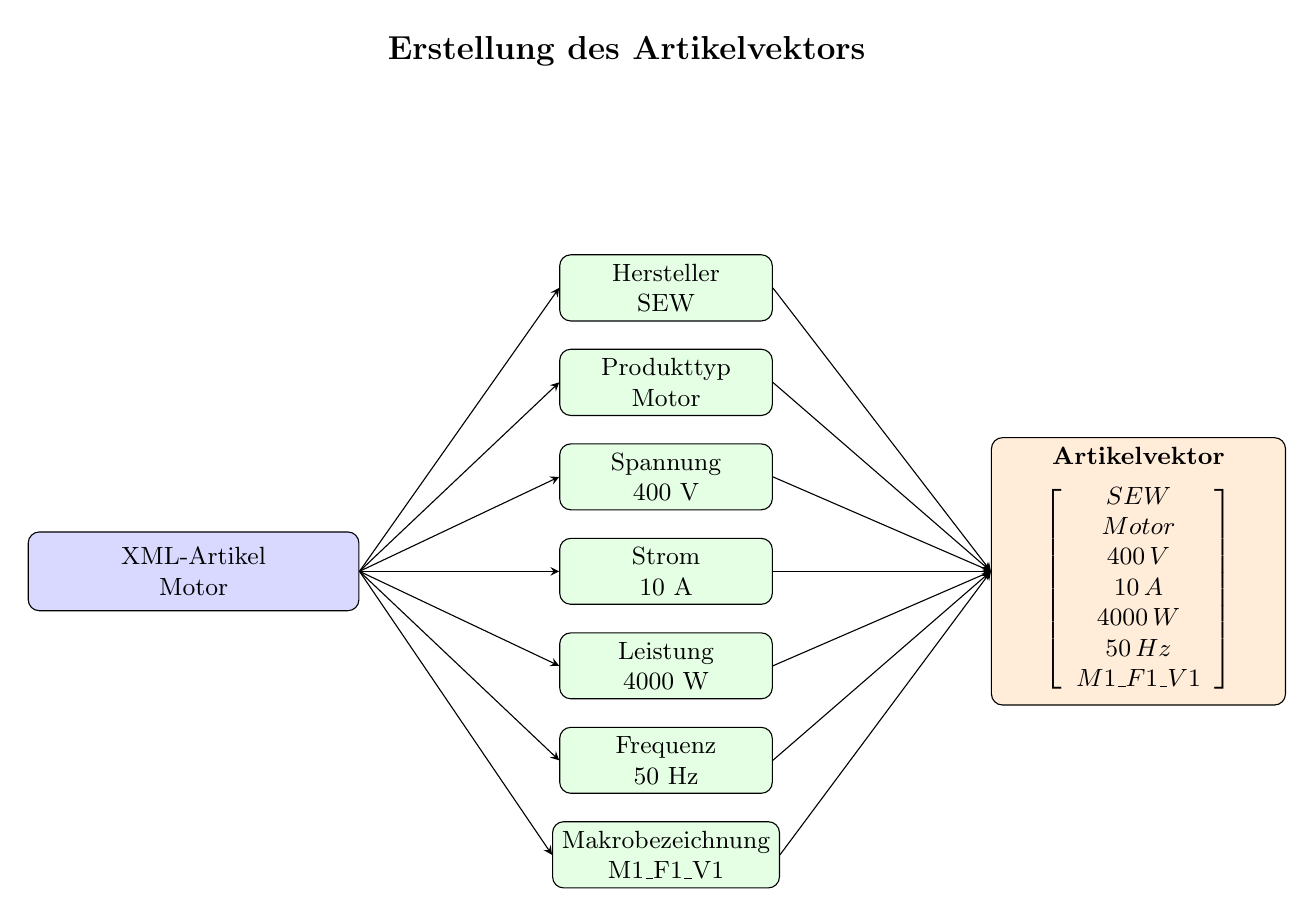
\begin{tikzpicture}[ >=stealth, font=\small, 
        source/.style={ draw, rounded corners, fill=blue!15, minimum width=4.2cm, minimum height=1cm, align=center }, 
        feature/.style={ draw, rounded corners, fill=green!10, minimum width=2.7cm, minimum height=0.8cm, align=center }, 
        vector/.style={ draw, rounded corners, fill=orange!15, minimum width=11cm, minimum height=1cm, align=left } ] 
        
        %%%%%%%%%%%%%%%%%%%%%%%%%%%%%%%%%%%%%%%%%%%%%%%%% % Titel %%%%%%%%%%%%%%%%%%%%%%%%%%%%%%%%%%%%%%%%%%%%%%%%% 
        
        \node[font=\bfseries\large] at (-1.5,5) {Erstellung des Artikelvektors}; 

        
        %%%%%%%%%%%%%%%%%%%%%%%%%%%%%%%%%%%%%%%%%%%%%%%%% % Quelle %%%%%%%%%%%%%%%%%%%%%%%%%%%%%%%%%%%%%%%%%%%%%%%%% 
        \node[source] (article) at (-7,-1.6) {XML-Artikel\\Motor}; 
        
        %%%%%%%%%%%%%%%%%%%%%%%%%%%%%%%%%%%%%%%%%%%%%%%%% % Merkmale %%%%%%%%%%%%%%%%%%%%%%%%%%%%%%%%%%%%%%%%%%%%%%%%% 
        \node[feature] (manufacturer) at (-1,2) {Hersteller\\SEW}; 
        \node[feature] (type) at (-1,0.8) {Produkttyp\\Motor}; 
        \node[feature] (voltage) at (-1,-0.4) {Spannung\\400 V}; 
        \node[feature] (current) at (-1,-1.6) {Strom\\10 A}; 
        \node[feature] (power) at (-1,-2.8) {Leistung\\4000 W}; 
        \node[feature] (frequency) at (-1,-4) {Frequenz\\50 Hz};
        \node[feature] (macro) at (-1,-5.2) {Makrobezeichnung\\M1\_F1\_V1};
        
        %%%%%%%%%%%%%%%%%%%%%%%%%%%%%%%%%%%%%%%%%%%%%%%%% % Verbindungen Quelle -> Features %%%%%%%%%%%%%%%%%%%%%%%%%%%%%%%%%%%%%%%%%%%%%%%%% 
        \draw[->] (article.east) -- (manufacturer.west); 
        \draw[->] (article.east) -- (type.west); 
        \draw[->] (article.east) -- (voltage.west); 
        \draw[->] (article.east) -- (current.west); 
        \draw[->] (article.east) -- (power.west); 
        \draw[->] (article.east) -- (frequency.west); 
        \draw[->] (article.east) -- (macro.west); 
        %%%%%%%%%%%%%%%%%%%%%%%%%%%%%%%%%%%%%%%%%%%%%%%%% % Artikelvektor %%%%%%%%%%%%%%%%%%%%%%%%%%%%%%%%%%%%%%%%%%%%%%%%% 
        \node[ draw, rounded corners, fill=orange!15, text width=3.5cm, align=center ] (vector) at (5,-1.6) { \textbf{Artikelvektor\\} \vspace{2mm} $ \left[ \begin{array}{c} SEW\\ Motor\\ 400\,V\\ 10\,A\\ 4000\,W\\ 50\,Hz\\ M1\_F1\_V1 \end{array} \right] $ }; 
        %%%%%%%%%%%%%%%%%%%%%%%%%%%%%%%%%%%%%%%%%%%%%%%%% % Verbindungen Features -> Vektor %%%%%%%%%%%%%%%%%%%%%%%%%%%%%%%%%%%%%%%%%%%%%%%%% 
        \draw[->] (manufacturer.east) -- (vector.west); 
        \draw[->] (type.east) -- (vector.west); 
        \draw[->] (voltage.east) -- (vector.west); 
        \draw[->] (current.east) -- (vector.west); 
        \draw[->] (power.east) -- (vector.west);
        \draw[->] (frequency.east) -- (vector.west);
        \draw[->] (macro.east) -- (vector.west);
    \end{tikzpicture} 
    \caption{Erzeugung eines Artikelvektors aus \textit{technischen Artikeleigenschaften} eines Motorartikels. Die extrahierten Merkmale werden zu einer gemeinsamen technischen Repräsentation zusammengeführt und dienen als Eingabe für das Empfehlungssystem.} 
    \label{fig:artikelvektor} 
\end{figure}
        
\subsection{Makrovektor}
\label{sec:makrovektor} 

Der Makrovektor stellt analog zum Artikelvektor folgende \textit{technische Makroeigenschaften} in einem gemeinsamen Vektor zusammengeführt dar: 

\begin{itemize} 
    \item Anschlüsse, 
    \item Makrokategorien, 
    \item Familien, 
    \item Varianten, 

\end{itemize} 

Im Bezug auf das Motorbeispiel zeigt folgende Abbildung \ref{fig:makrovektor} den Aufbau des Makrovektors:

\begin{figure}[H] 
    \centering 
    \begin{tikzpicture}[ >=stealth, font=\small, 
        source/.style={ draw, rounded corners, fill=blue!15, minimum width=4cm, minimum height=1.2cm, align=center }, 
        feature/.style={ draw, rounded corners, fill=green!10, minimum width=3cm, minimum height=0.8cm, align=center }, 
        vector/.style={ draw, rounded corners, fill=orange!15, minimum width=4cm, minimum height=3.5cm, align=left } ] 
        
        %%%%%%%%%%%%%%%%%%%%%%%%%%%%%%%%%%%%%%%%%%%%%%%%% % Titel %%%%%%%%%%%%%%%%%%%%%%%%%%%%%%%%%%%%%%%%%%%%%%%%% 
        
        \node[font=\bfseries\large] at (-1,5) {Erstellung des Makrovektors}; 
        
        %%%%%%%%%%%%%%%%%%%%%%%%%%%%%%%%%%%%%%%%%%%%%%%%% % Quelle %%%%%%%%%%%%%%%%%%%%%%%%%%%%%%%%%%%%%%%%%%%%%%%%% 
        
        \node[source] (macro) at (-7,0) {.ema-Makro\\Motor}; 
        
        %%%%%%%%%%%%%%%%%%%%%%%%%%%%%%%%%%%%%%%%%%%%%%%%% % Features %%%%%%%%%%%%%%%%%%%%%%%%%%%%%%%%%%%%%%%%%%%%%%%%% 
        
        \node[feature] (terminal) at (-1,2) {Anschlüsse\\U1, V1, W1}; 
        \node[feature] (category) at (-1,0.8) {Kategorie\\Motor}; 
        \node[feature] (family) at (-1,-0.4) {Familie\\F1}; 
        \node[feature] (variant) at (-1,-1.6) {Variante\\Mit Kühlung}; 
    
        %%%%%%%%%%%%%%%%%%%%%%%%%%%%%%%%%%%%%%%%%%%%%%%%% % Verbindungen Quelle -> Features %%%%%%%%%%%%%%%%%%%%%%%%%%%%%%%%%%%%%%%%%%%%%%%%% 
        
        \draw[->] (macro.east) -- (terminal.west); \draw[->] (macro.east) -- (category.west); 
        \draw[->] (macro.east) -- (family.west); \draw[->] (macro.east) -- (variant.west); 
        
        %%%%%%%%%%%%%%%%%%%%%%%%%%%%%%%%%%%%%%%%%%%%%%%%% % Vektor %%%%%%%%%%%%%%%%%%%%%%%%%%%%%%%%%%%%%%%%%%%%%%%%% 

        \node[ draw, rounded corners, fill=orange!15, text width=3.5cm, align=center ] (vector) at (5,0) { \textbf{Makrovektor\\} \vspace{2mm} $\left[\! \begin{array}{c} U1,V1,W1\\ Motor\\ F1\\ \text{Mit Kühlung} \end{array} \!\right]$ };

        %%%%%%%%%%%%%%%%%%%%%%%%%%%%%%%%%%%%%%%%%%%%%%%%% % Verbindungen Features -> Vektor %%%%%%%%%%%%%%%%%%%%%%%%%%%%%%%%%%%%%%%%%%%%%%%%% 
        \draw[->] (terminal.east) -- (vector.west); 
        \draw[->] (category.east) -- (vector.west); 
        \draw[->] (family.east) -- (vector.west); 
        \draw[->] (variant.east) -- (vector.west); 
        \end{tikzpicture} 
        \caption{Erstellung des Makrovektor. Aus dem .ema-Makro werden strukturelle Informationen extrahiert und in einen Vektor überführt, der die technische Struktur des Makros für das Empfehlungssystem beschreibt.} 
        \label{fig:makrovektor} 
        \end{figure}

\subsection{Lexikalvektor} 

Nicht alle \textit{technischen Artikel- und Makroeigenschaften} liegen in Form von konkreten Werten wie zum Beispiel 24 V in den vorhandenen Artikeldaten vor. Technische Hinweise in einem Artikelliegen in Textform vor. 
Diese \textit{technischen Hinweise} stellen aufgrund der Textform eine andere Art von \textit{technischen Artikeleigenschaften} dar als solche mit konkreten Werten \cite{baltrusaitis2019multimodal}.
Hierdurch können Informationen genutzt werden, die in Zahlen nicht abbildbar sind, wie zum Beispiel die wasserdichte Ausführung eines Motors.
Diese textbasierten \textit{technischen Artikeleigenschaften} stellen somit eine weitere Information dar, welche Gemeinsamkeiten und Unterschiede zwischen Artikeln aufzeigen.
Die folgende Abbildung \ref{fig:lexikalische_information_empfehlung} zeigt, welchen Einfluss \textit{technischen Hinweise} auf die Unterscheidung von Artikeln haben: 

\begin{figure}[H] 
    \centering 
    \begin{tikzpicture}[ >=stealth, font=\small, 
        query/.style={ draw, rounded corners, fill=blue!15, text width=5.2cm, minimum height=3.8cm, align=left, inner sep=7pt }, 
        candidate/.style={ draw, rounded corners, fill=gray!10, text width=4.8cm, minimum height=4.3cm, align=left, inner sep=7pt }, 
        match/.style={ draw, rounded corners, fill=green!10, text width=4.4cm, minimum height=1.1cm, align=center, inner sep=5pt }, 
        mismatch/.style={ draw, rounded corners, fill=red!10, text width=4.4cm, minimum height=1.1cm, align=center, inner sep=5pt }, 
        decision/.style={ draw, rounded corners, fill=yellow!20, text width=5.8cm, minimum height=1.4cm, align=center, inner sep=7pt }, 
        result/.style={ draw, rounded corners, fill=green!15, text width=6cm, minimum height=1.5cm, align=center, inner sep=7pt } ] 
        
        %%%%%%%%%%%%%%%%%%%%%%%%%%%%%%%%%%%%%%%%%%%%%%%%% % Titel %%%%%%%%%%%%%%%%%%%%%%%%%%%%%%%%%%%%%%%%%%%%%%%%% \
        
        node[font=\bfseries\large] at (0,11) {Einfluss textbasierter Informationen auf die Makroempfehlung}; 
        
        %%%%%%%%%%%%%%%%%%%%%%%%%%%%%%%%%%%%%%%%%%%%%%%%% % Anfrage %%%%%%%%%%%%%%%%%%%%%%%%%%%%%%%%%%%%%%%%%%%%%%%%% 
        
        \node[query] (request) at (0,8.2) { \centering \textbf{Anfrage}\\[2mm] \raggedright Artikel: Elektromotor\\ Hersteller: Siemens\\ Spannung: 400 V\\ Strom: 10 A\\[1mm] \textbf{Anmerkung:}\\ \textbf{Wasserdichte Ausführung} }; 
        
        %%%%%%%%%%%%%%%%%%%%%%%%%%%%%%%%%%%%%%%%%%%%%%%%% % Verzweigung der Kandidatensuche %%%%%%%%%%%%%%%%%%%%%%%%%%%%%%%%%%%%%%%%%%%%%%%%% 
        
        \coordinate (branch) at (0,5.7); \draw[->,thick] (request.south) -- (branch); 
        \node[ fill=white, inner sep=3pt, font=\bfseries ] at (0,6.1) {Vergleich mit vorhandenen Artikeln}; 
        
        %%%%%%%%%%%%%%%%%%%%%%%%%%%%%%%%%%%%%%%%%%%%%%%%% % Artikel A und Artikel B %%%%%%%%%%%%%%%%%%%%%%%%%%%%%%%%%%%%%%%%%%%%%%%%% 
        
        \node[candidate] (articleA) at (-4.2,2.8) { \centering \textbf{Artikel A}\\[2mm] \raggedright Artikel: Elektromotor\\ Hersteller: Siemens\\ Spannung: 400 V\\ Strom: 10 A\\[1mm] \textbf{Anmerkung:}\\ \textbf{Wasserdichte Ausführung}\\[1mm] Makro: M1\_F1\_V1 }; 
        \node[candidate] (articleB) at (4.2,2.8) { \centering \textbf{Artikel B}\\[2mm] \raggedright Artikel: Elektromotor\\ Hersteller: Siemens\\ Spannung: 400 V\\ Strom: 10 A\\[1mm] \textbf{Anmerkung:}\\ keine Angabe\\[1mm] Makro: M1\_F1\_V2 }; 
        
        % Klare, symmetrische Verbindungen \draw[->,thick] (branch) -| (articleA.north); \draw[->,thick] (branch) -| (articleB.north); 
        
        %%%%%%%%%%%%%%%%%%%%%%%%%%%%%%%%%%%%%%%%%%%%%%%%% % Bewertung der Kandidaten %%%%%%%%%%%%%%%%%%%%%%%%%%%%%%%%%%%%%%%%%%%%%%%%% 
        
        \node[match] (matchA) at (-4.2,-1.3) { \textbf{Hohe Übereinstimmung}\\ Anmerkung vorhanden }; 
        \node[mismatch] (matchB) at (4.2,-1.3) { \textbf{Geringere Übereinstimmung}\\ Anmerkung fehlt }; 
        
        \draw[->,thick,green!50!black] (articleA.south) -- (matchA.north); \draw[->,thick,red!70!black] (articleB.south) -- (matchB.north); 
        
        %%%%%%%%%%%%%%%%%%%%%%%%%%%%%%%%%%%%%%%%%%%%%%%%% % Gemeinsame Entscheidung %%%%%%%%%%%%%%%%%%%%%%%%%%%%%%%%%%%%%%%%%%%%%%%%% 
        
        \node[decision] (decision) at (0,-4.3) { \textbf{Entscheidender \textit{technischer Hinweis} }\\[1mm] „Wasserdichte Ausführung“ }; \draw[->,thick,green!50!black] (matchA.south) |- (decision.west); \draw[->,thick,red!70!black] (matchB.south) |- (decision.east); 
        
        %%%%%%%%%%%%%%%%%%%%%%%%%%%%%%%%%%%%%%%%%%%%%%%%% % Empfehlung %%%%%%%%%%%%%%%%%%%%%%%%%%%%%%%%%%%%%%%%%%%%%%%%% 
        
        \node[result] (recommendation) at (0,-7) { \textbf{Empfehlung: Makro M1\_F1\_V1}\\[1mm] Artikel A besitzt die größere Gesamtübereinstimmung. }; 
        \draw[->,very thick,green!50!black] (decision.south) -- (recommendation.north); 
    \end{tikzpicture} 
    \caption{Einfluss einer textbasierten technischen Information auf die Makroempfehlung. Artikel A und B sind bis auf die Anmerkung „Wasserdichte Ausführung“ identisch. Dadurch wird Artikel A bevorzugt, sodass das zugeordnete Makro M1\_F1\_V1 empfohlen wird. } 
    \label{fig:lexikalische_information_empfehlung} 
\end{figure}

Aus den vorhandenen Artikeldaten lassen sich folgende textbasierten \textit{technischen Artikeleigenschaften} extrahieren: 

\begin{itemize} 
    \item Typbezeichnungen, 
    \item Produktserien, 
    \item technischen Beschreibungen. 
\end{itemize} 

Abbildung \ref{fig:lexikalvektor} stellt den Aufbau des Lexikalvektors für das Beispiel des Motors dar:

\begin{figure}[H] 
    \centering 
    \begin{tikzpicture}[ >=stealth, font=\small, 
        source/.style={ draw, rounded corners, fill=blue!15, minimum width=4cm, minimum height=1.2cm, align=center }, 
        feature/.style={ draw, rounded corners, fill=green!10, minimum width=3.0cm, minimum height=0.8cm, align=center } ] 
        
        %%%%%%%%%%%%%%%%%%%%%%%%%%%%%%%%%%%%%%%%%%%%%%%%% % Titel %%%%%%%%%%%%%%%%%%%%%%%%%%%%%%%%%%%%%%%%%%%%%%%%% 
        
        \node[font=\bfseries\large] at (-1,5) {Erstellung des Lexikalvektors}; 
        
        %%%%%%%%%%%%%%%%%%%%%%%%%%%%%%%%%%%%%%%%%%%%%%%%% % Quellen %%%%%%%%%%%%%%%%%%%%%%%%%%%%%%%%%%%%%%%%%%%%%%%%% 
        
        \node[source] (article) at (-7,0.5) {XML-Artikel\\Motor};  
        
        %%%%%%%%%%%%%%%%%%%%%%%%%%%%%%%%%%%%%%%%%%%%%%%%% % Lexikalische Merkmale %%%%%%%%%%%%%%%%%%%%%%%%%%%%%%%%%%%%%%%%%%%%%%%%% 
        
        \node[feature] (type) at (-1,2.5) {Typbezeichnung\\DRN112M4}; 
        \node[feature] (series) at (-1,0.5) {Produktserie\\DRN}; 
        \node[feature] (description) at (-1,-1.0) {Beschreibung\\Wasserdichte Ausführung}; 
        %%%%%%%%%%%%%%%%%%%%%%%%%%%%%%%%%%%%%%%%%%%%%%%%% % Quelle -> Merkmale %%%%%%%%%%%%%%%%%%%%%%%%%%%%%%%%%%%%%%%%%%%%%%%%% 
        
        \draw[->] (article.east) -- (type.west); 
        \draw[->] (article.east) -- (series.west); 
        \draw[->] (article.east) -- (description.west); 
        
        %%%%%%%%%%%%%%%%%%%%%%%%%%%%%%%%%%%%%%%%%%%%%%%%% % Lexikalvektor %%%%%%%%%%%%%%%%%%%%%%%%%%%%%%%%%%%%%%%%%%%%%%%%% 
        
        \node[ draw, rounded corners, fill=orange!15, text width=5cm, align=center ] (vector) at (5,0.5) { \textbf{Lexikalvektor\\} \vspace{2mm} $\left[ \begin{array}{c} \text{DRN112M4}\\ \text{DRN}\\ \text{Wasserdichte Ausführung} \end{array} \right]$ };
        
        %%%%%%%%%%%%%%%%%%%%%%%%%%%%%%%%%%%%%%%%%%%%%%%%% % Merkmale -> Vektor %%%%%%%%%%%%%%%%%%%%%%%%%%%%%%%%%%%%%%%%%%%%%%%%% 
        \draw[->] (type.east) -- (vector.west); 
        \draw[->] (series.east) -- (vector.west); 
        \draw[->] (description.east) -- (vector.west); 
        \end{tikzpicture} 
        \caption{Erstellung des Lexikalvektors. Textuelle technische Informationen aus Artikel- und Makrodaten werden extrahiert und in einem separaten Vektor zusammengeführt. 
        Der Lexikalvektor ergänzt die strukturierten Informationen des Artikel- und Makrovektors um technische Begriffe und Bezeichnungen.} 
        \label{fig:lexikalvektor} 
        \end{figure}

\subsection{Warum Drei Vektoren ?}

Die Aufteilung der \textit{technischen Artikel- und Makroeigenschaften} in drei separate Vektoren hat mehrere Vorteile:

%%%%%%% Argumentation Anpassen ! %%%%%%%

% \begin{itemize}
%     \item Es wird verhindert, dass sich Werte aus den Artikel- und Makrodaten wie Spannung, Strom oder Makrobezeichnungen mit textuellen \textit{technischen Artikel- und Makroeigenschaften} aus den Hinweis- und Beschreibungsfeldern vermischen. Eine Spannung von 400 V besitzt eine andere Bedeutung als der Hinweis "Wasserdichte Ausführung". Durch die getrennte Speicherung bleiben diese unterschiedlichen Informationsarten für ein späteres Modell unterscheidbar. Dies folgt dem Konzept der multimodaler Datenrepräsentationen wie in \cite{baltrusaitis2019multimodal} und \cite{ebrahimi2024lanistr} beschrieben.
%     \item Die Weiterentwicklung der einzelnen Informationsquellen ist unabhängig voneinander möglich. Neue technische Merkmale können beispielsweise dem Artikelvektor hinzugefügt werden, ohne die Struktur des Makrovektors oder des Lexikalvektors verändern zu müssen. 
%     \item Zusätzlich können die einzelnen Vektoren später unterschiedlich verarbeitet werden. Strukturierte \textit{technische Eigenschaften} des Artikel- und Makrovektors können beispielsweise direkt als numerische Eingaben für Learning-to-Rank-Verfahren verwendet werden, während textuelle \textit{technische Eigenschaften} des Lexikalvektors zusätzlich durch Embedding-Modelle oder Sentence Transformer verarbeitet werden können (siehe Kapitel \ref{sec:modellansätze}).
% \end{itemize}
 

\section{Erstellung des Datensplits} 
\subsection{Trainings-, Validierungs- und Testdaten}

Ein Datensplit (Abbildung \ref{fig:datensplit_funktion}) ist die Aufteilung eines Datensatzes in voneinander getrennte Teilmengen, den Trainings-, Validierungs- und Testdaten. 
Dabei dienen die Trainingsdaten dem Lernprozess des Modells, wodurch die Zusammenhänge zwischen den \textit{technischen Artikel- und Makroeigenschaften} erlernt werden. 
Die Validierungsdaten werden verwendet, um die Parameter des Modells während des Lernprozesses zu überwachen und anzupassen. 
Die Testdaten dienen der abschließenden Bewertung des Modells, um dessen Leistungsfähigkeit auf unbekannte Artikeldaten zu überprüfen \cite{kohavi1995cv,hastie2009elements}.

\begin{figure}[H] 
    \centering 
    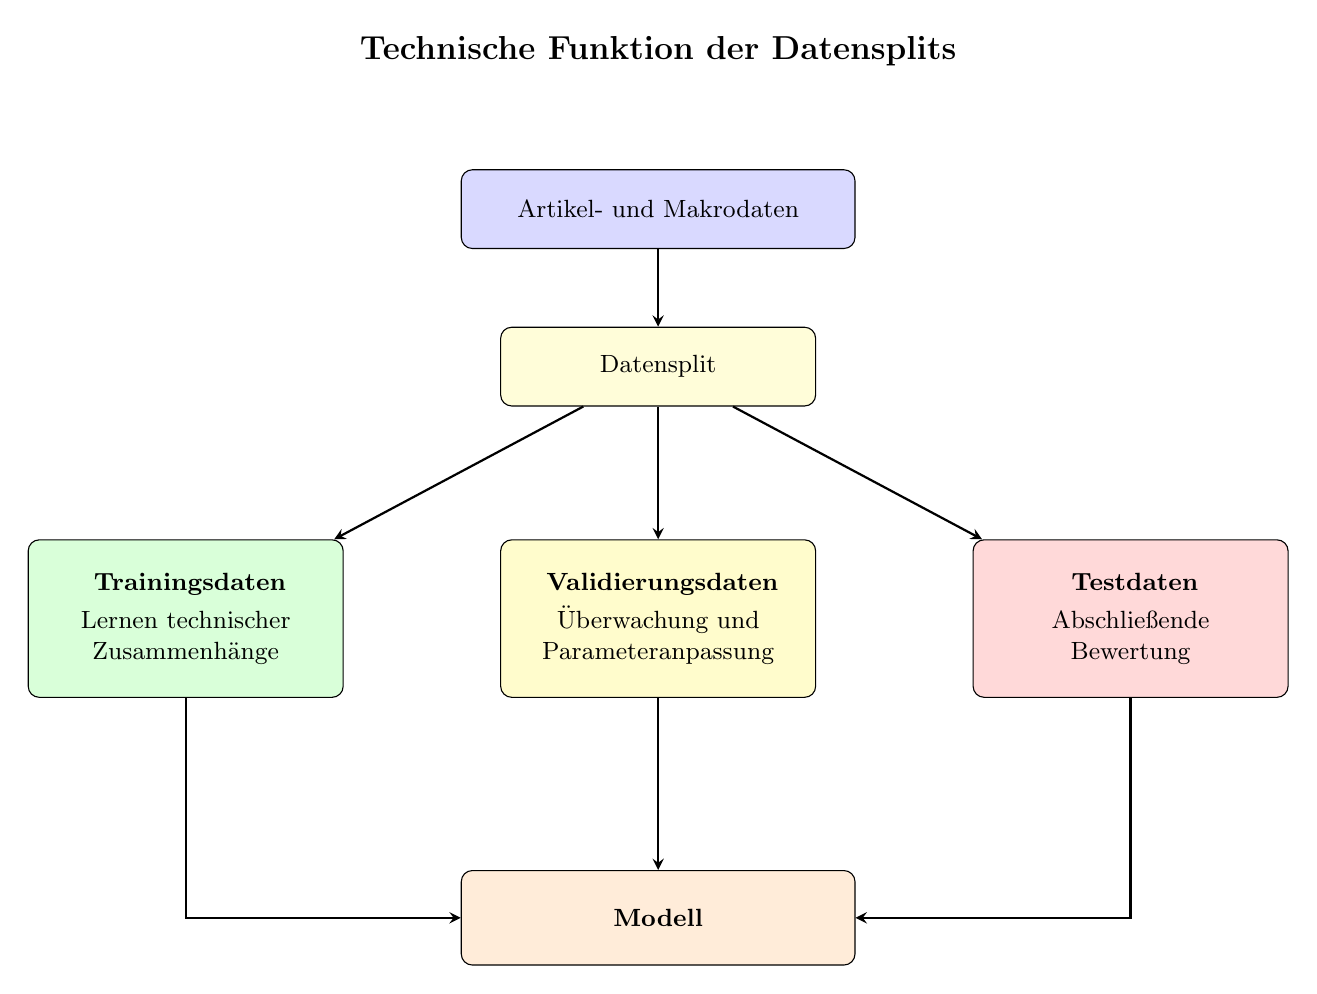
\begin{tikzpicture}[ >=stealth, font=\small, 
        dataset/.style={ draw, rounded corners, fill=blue!15, minimum width=5cm, minimum height=1cm, align=center }, 
        split/.style={ draw, rounded corners, minimum width=4cm, minimum height=2cm, align=center }, 
        model/.style={ draw, rounded corners, fill=orange!15, minimum width=5cm, minimum height=1.2cm, align=center } ] 
        
        %%%%%%%%%%%%%%%%%%%%%%%%%%%%%%%%%%%%%%%%%%%%%%%%% % Titel %%%%%%%%%%%%%%%%%%%%%%%%%%%%%%%%%%%%%%%%%%%%%%%%% 
        
        \node[font=\bfseries\large] at (0,7) {Technische Funktion der Datensplits}; 
        
        %%%%%%%%%%%%%%%%%%%%%%%%%%%%%%%%%%%%%%%%%%%%%%%%% % Datenbasis %%%%%%%%%%%%%%%%%%%%%%%%%%%%%%%%%%%%%%%%%%%%%%%%% 
        
        \node[dataset] (data) at (0,5) {Artikel- und Makrodaten}; 
        
        %%%%%%%%%%%%%%%%%%%%%%%%%%%%%%%%%%%%%%%%%%%%%%%%% % Datensplit %%%%%%%%%%%%%%%%%%%%%%%%%%%%%%%%%%%%%%%%%%%%%%%%% 
        
        \node[ draw, rounded corners, fill=yellow!15, minimum width=4cm, minimum height=1cm ] (split) at (0,3) {Datensplit}; 
        \draw[->,thick] (data) -- (split); 
        
        %%%%%%%%%%%%%%%%%%%%%%%%%%%%%%%%%%%%%%%%%%%%%%%%% % Trainingsdaten %%%%%%%%%%%%%%%%%%%%%%%%%%%%%%%%%%%%%%%%%%%%%%%%% 
        
        \node[ split, fill=green!15, text width=3.5cm ] (train) at (-6,-0.2) { \vspace{1mm} \textbf{Trainingsdaten} Lernen technischer Zusammenhänge }; 
        
        %%%%%%%%%%%%%%%%%%%%%%%%%%%%%%%%%%%%%%%%%%%%%%%%% % Validierung %%%%%%%%%%%%%%%%%%%%%%%%%%%%%%%%%%%%%%%%%%%%%%%%% 
        
        \node[ split, fill=yellow!20, text width=3.5cm ] (val) at (0,-0.2) {  \vspace{1mm} \textbf{Validierungsdaten} Überwachung und Parameteranpassung }; 
        
        %%%%%%%%%%%%%%%%%%%%%%%%%%%%%%%%%%%%%%%%%%%%%%%%% % Test %%%%%%%%%%%%%%%%%%%%%%%%%%%%%%%%%%%%%%%%%%%%%%%%% 
        
        \node[ split, fill=red!15, text width=3.5cm ] (test) at (6,-0.2) { \vspace{1mm} \textbf{Testdaten\\} Abschließende Bewertung }; 
        
        %%%%%%%%%%%%%%%%%%%%%%%%%%%%%%%%%%%%%%%%%%%%%%%%% % Aufteilung %%%%%%%%%%%%%%%%%%%%%%%%%%%%%%%%%%%%%%%%%%%%%%%%% 
        
        \draw[->,thick] (split) -- (train); \draw[->,thick] (split) -- (val); \draw[->,thick] (split) -- (test); 
        
        %%%%%%%%%%%%%%%%%%%%%%%%%%%%%%%%%%%%%%%%%%%%%%%%% % Modell %%%%%%%%%%%%%%%%%%%%%%%%%%%%%%%%%%%%%%%%%%%%%%%%% 
        
        \node[ draw, rounded corners, fill=orange!15, minimum width=5cm, minimum height=1.2cm, align=center ] (model) at (0,-4) { \vspace{2mm} \textbf{Modell} };
        
        %%%%%%%%%%%%%%%%%%%%%%%%%%%%%%%%%%%%%%%%%%%%%%%%% % Datenfluss %%%%%%%%%%%%%%%%%%%%%%%%%%%%%%%%%%%%%%%%%%%%%%%%% 
        
        \draw[->,thick] (train.south) |- (model.west); 
        \draw[->,thick] (val.south) -- (model.north); 
        \draw[->,thick] (test.south) |- (model.east); 
        \end{tikzpicture} 
        \caption{Technische Funktion der Trainings-, Validierungs- und Testdaten. Während die Trainingsdaten für das Erlernen technischer Zusammenhänge genutzt werden, dienen die Validierungsdaten der Überwachung und Anpassung des Modells. Die Testdaten werden ausschließlich zur abschließenden Bewertung der Leistungsfähigkeit auf unbekannten Daten verwendet.} 
        \label{fig:datensplit_funktion} 
        \end{figure}


\subsection{Splitregeln und deren Ergebnis}
\label{sec:splitregeln} 

Die Herausforderung aus der Datenaufbereitung (siehe Abschnitt \ref{sec:ergebnis_der_datenaufbereitung}) soll in diesem Abschnitt durch die Festlegung von Splitregeln für die Trainings-, Validierungs- und Testdaten adressiert werden.
Dabei ist zu beachten, dass Artikel und Makro in einer n:1-Beziehung stehen (siehe Kapitel \ref{sec:artikel_macro_zuordnungen}), das heißt, es können mehrere Artikel demselben Makro zugeordnet werden. Daraus lassen sich die folgenden Splitregeln ableiten: 

\begin{itemize} 
    \item Regel 1: Ein Makro muss immer durch mindestens einen Artikel in den Trainingsdaten vertreten sein. 
    \item Regel 2: Ein Makro, das mit einem Artikel in den Testdaten vorkommt, muss mindestens einen Artikel in den Trainingsdaten besitzen. 
    \item Regel 3: Ein Makro, das in den Validierungsdaten vorkommt, muss mindestens einen Artikel in den Trainings- und Testdaten besitzen. 
    \item Regel 4: Es dürfen keine identischen Artikel gleichzeitig in Trainings-, Validierungs- und Testdaten vorkommen. 
\end{itemize} 

Alle Artikel- und Makrodaten, welche in den Validierungs- oder Testdaten vorkommen, müssen im Trainingsbestand vertreten sein, da fehlende Trainingsdaten die Bewertung des Modells verfälschen würden. 
Angenommen ein Makro kommt in den Validierungs- oder Testdaten vor, aber nicht in den Trainingsdaten. Die Bewertung für dieses Makro ist dann fehlerhaft, da ein Makro bewertet wird, zu dem das Modell kein Wissen besitzt.

Unter Berücksichtigung der definierten Splitregeln und auf Grundlage des Datenbestands aus Abschnitt \ref{sec:ergebnis_der_datenaufbereitung} sowie der zuvor beschriebenen Datenaufbereitung ergibt sich der folgende Datensplit: 

\begin{itemize} 
\item 1.300 Trainingsartikel (83,4\,\%), 
\item 96 Validierungsartikel (6,2\,\%), 
\item 163 Testartikel (10,4\,\%). 
\end{itemize}

Dieser Datensplit bildet die Basis für das Training und die Bewertung des Modells.

\section{Artefakt A1: Trainings- und Evaluationsbasis} 

Ziel dieses Kapitels war die Beantwortung der Forschungsfrage RQ1: 

\begin{quote} 
    \textbf{RQ1:} Welche technischen Informationen aus Artikeln eignen sich zur Unterscheidung von Makros und können als Trainings- und Evaluationsbasis für ein Empfehlungssystem verwendet werden? 
\end{quote} 

Zur Beantwortung dieser Forschungsfrage wurden zunächst die verfügbaren Artikel-, Makro- und Zuordnungsdaten analysiert. 
Anschließend erfolgte eine mehrstufige Datenaufbereitung bestehend aus der Entfernung unvollständiger Datensätze, der Entfernung redundanter Artikel, 
der Bereinigung nicht nutzbarer Metadaten sowie der Normalisierung und Klassifikation technischer Eigenschaften. 
Auf Basis der bereinigten Daten wurden die relevanten technischen Informationen in ein maschinell verarbeitbares Format überführt. 
Hierzu wurden die technischen Artikeleigenschaften in Form von Artikelvektoren repräsentiert und anschließend in Trainings-, Validierungs- und Testdaten aufgeteilt. 
Das Ergebnis dieser Schritte stellt die Trainings- und Evaluationsbasis des späteren Empfehlungssystems dar und bildet damit die Grundlage für die Auswahl und Bewertung geeigneter Modellansätze im nachfolgenden Kapitel. 

Daraus ergibt sich folgendes Artefakt, dass an die nächsten Kapitel übergeben wird: 

\begin{quote} 
    \textbf{Artefakt A1: Trainings- und Evaluationsbasis} 
\end{quote} 
\begin{itemize} 
    \item 1.559 aufbereitete Artikel,
    \item 375 unterschiedliche Makros,
    \item 127 \textit{technischen Artikeleigenschaften},
    \item Artikel-Makro-Zuordnungen,
    \item normalisierte und klassifizierte \textit{technischen Artikeleigenschaften},
    \item Artikelvektoren als maschinenlesbare Repräsentation der Artikel,
    \item Datensplit bestehend aus: 
    \begin{itemize} 
        \item 1.300 Trainingsartikeln
        \item 96 Validierungsartikeln
        \item 163 Testartikeln
    \end{itemize} 
\end{itemize} 



% \subsection{Architektur der Datenanalyse und Trainingsvorbereitung} 

% \begin{figure}[H] 
%     \centering 
%     \begin{tikzpicture}[ >=stealth, font=\small, 
%         source/.style={ draw, rounded corners, fill=blue!15, minimum width=3.8cm, minimum height=1cm, align=center }, 
%         process/.style={ draw, rounded corners, fill=green!15, minimum width=4.5cm, minimum height=1.1cm, align=center }, 
%         artifact/.style={ draw, rounded corners, fill=orange!15, minimum width=5.0cm, minimum height=1cm, align=center } ] 
        
%         %%%%%%%%%%%%%%%%%%%%%%%%%%%%%%%%%%%%%%%%%%%%%%%%% % Datenbasis %%%%%%%%%%%%%%%%%%%%%%%%%%%%%%%%%%%%%%%%%%%%%%%%% 
        
%         \node[source] (article) at (-5,10) {XML-Artikeldaten}; 
%         \node[source] (macro) at (5,10) {EMA-Makrodaten}; 
%         \node[source] (mapping) at (0,10) {Artikel-Makro\\Zuordnungen}; 
        
%         %%%%%%%%%%%%%%%%%%%%%%%%%%%%%%%%%%%%%%%%%%%%%%%%% % Datenaufbereitung %%%%%%%%%%%%%%%%%%%%%%%%%%%%%%%%%%%%%%%%%%%%%%%%% 
        
%         \node[process] (prepare) at (0,7.5) { \vspace{2mm} \textbf{Datenaufbereitung}\\ Bereinigung\\ Normalisierung\\ Klassifikation }; 
%         \draw[->,thick] (article) -- (prepare); 
%         \draw[->,thick] (macro) -- (prepare); 
%         \draw[->,thick] (mapping) -- (prepare); 
        
%         %%%%%%%%%%%%%%%%%%%%%%%%%%%%%%%%%%%%%%%%%%%%%%%%% % Übergabeartefakt %%%%%%%%%%%%%%%%%%%%%%%%%%%%%%%%%%%%%%%%%%%%%%%%% 
        
%         \node[artifact] (features) at (0,5.0) { \vspace{2mm} \textbf{Übergabeartefakt}\\ Geprüfte Datenbasis }; 
%         \draw[->,thick] (prepare) -- (features); 
        
%         %%%%%%%%%%%%%%%%%%%%%%%%%%%%%%%%%%%%%%%%%%%%%%%%% % Trainingsformat %%%%%%%%%%%%%%%%%%%%%%%%%%%%%%%%%%%%%%%%%%%%%%%%% 
        
%         \node[process] (vectorize) at (0,2.4) { \vspace{2mm} \textbf{Überführung in Trainingsformat}\\ Merkmalsextraktion\\ Vektorisierung }; 
%         \draw[->,thick] (features) -- (vectorize); 
        
%         %%%%%%%%%%%%%%%%%%%%%%%%%%%%%%%%%%%%%%%%%%%%%%%%% % Vektoren %%%%%%%%%%%%%%%%%%%%%%%%%%%%%%%%%%%%%%%%%%%%%%%%% 
        
%         \node[artifact] (articlevec) at (-6,-0.5) {Artikelvektor}; 
%         \node[artifact] (macrovec) at (0,-0.5) {Makrovektor}; 
%         \node[artifact] (lexicalvec) at (6,-0.5) {Lexikalvektor}; 
%         \draw[->,thick] (vectorize) -- (articlevec); \draw[->,thick] (vectorize) -- (macrovec); 
%         \draw[->,thick] (vectorize) -- (lexicalvec); 
        
%         %%%%%%%%%%%%%%%%%%%%%%%%%%%%%%%%%%%%%%%%%%%%%%%%% % Datensplit %%%%%%%%%%%%%%%%%%%%%%%%%%%%%%%%%%%%%%%%%%%%%%%%% 
        
%         \node[process] (split) at (0,-3) { \vspace{2mm} \textbf{Datensplit}\\ Trainingsmenge: 1.300 Artikel\\ Validierungsmenge: 96 Artikel\\ Testmenge: 163 }; 
%         \draw[->,thick] (articlevec) |- (split); \draw[->,thick] (macrovec) -- (split); \draw[->,thick] (lexicalvec) |- (split); 
        
%         %%%%%%%%%%%%%%%%%%%%%%%%%%%%%%%%%%%%%%%%%%%%%%%%% % Split %%%%%%%%%%%%%%%%%%%%%%%%%%%%%%%%%%%%%%%%%%%%%%%%% 
        
%         \node[artifact] (train) at (-6,-6) { \vspace{2mm} \textbf{Training}\\1.300 Artikel}; 
%         \node[artifact] (val) at (0,-6) { \vspace{2mm} \textbf{Validierung}\\96 Artikel}; 
%         \node[artifact] (test) at (6,-6) { \vspace{2mm} \textbf{Test}\\163 Artikel}; 
%         \draw[->,thick] (split) -- (train); \draw[->,thick] (split) -- (val); 
%         \draw[->,thick] (split) -- (test); 
        
%         %%%%%%%%%%%%%%%%%%%%%%%%%%%%%%%%%%%%%%%%%%%%%%%%% % Artefakt A1 %%%%%%%%%%%%%%%%%%%%%%%%%%%%%%%%%%%%%%%%%%%%%%%%% 
        
%         \node[ draw, rounded corners, fill=yellow!20, minimum width=9cm, minimum height=1.6cm, align=center ] (a1) at (0,-8.5) { Artefakt A1\\ 1559 Artikel\\ 375 Makros}; 
%         \draw[->,thick] (train.south) |- (a1.west); \draw[->,thick] (val.south) -- (a1.north); \draw[->,thick] (test.south) |- (a1.east); \end{tikzpicture} 
%         \caption{ Architektur der Datenanalyse und Trainingsvorbereitung.} 
%     \end{figure}

